%% Šablona pro psaní závěrečných prací FBMI ČVUT
% Upraveno na základě požadavků na závěrečné práce schválených dne 24.2.2020.
%
% Vytvořeno ve spolupráci členů BRAIN Teamu.
% 
% Šablonu pro vás upravil/a:    Ing. Václava Piorecká, Ph.D.
% Kontakt:                      vaclava.piorecka@fbmi.cvut.cz

\documentclass[a4paper,12pt]{article}   % Definice - velikost dokumentu, základní velikost písma, typ
\usepackage[a4paper, top=2.5cm, left=3.5cm, right=2.5cm, bottom=2.5cm]{geometry}		% nastavení okrajů

%% Přidání balíčků podporujících různé funkcionality - ZÁKLADNÍ
\usepackage{amsmath,float}				% balíček pro matiku
\usepackage[dvipsnames]{xcolor}
\usepackage{color}
\usepackage{footnote}					% poznámka pod čarou
\usepackage{url}						% url odkazy
\DeclareUrlCommand\url{\def\UrlLeft{<}\def\UrlRight{>} \urlstyle{same}}   % nastavení URL odkazů pro podle normy ČSN ISO 690

\usepackage{float}						% plovoucí prostředí
\usepackage[utf8]{inputenc}			    % kódování	
\usepackage[czech]{babel}				% čeština
\usepackage{enumerate}      			% seznamy 
\usepackage{amsfonts}      				% množiny Z,R,N dvojitě
\usepackage{amssymb}      				% znaky úhlu a tak
\usepackage[pdftex]{graphicx}
\usepackage{setspace}
\usepackage{multicol}					% tabulka, slučování sloupců
\usepackage{multirow}                   % tabulka, slučování řádků
\usepackage{fancyhdr}					% záhlaví a zápatí stránky
\usepackage{chngcntr}                   % číslování (číslování rovnic, obrázků dle kapitol)
\usepackage{array}                      % rozšíření práce s tabulkami
\usepackage{helvet}                     % předefinuje \sfdefault to uhv (pro úvodní stránku)
\usepackage[flushleft]{threeparttable}  % prostředí pro tabulky - přidává vysvětlující poznámky pod tabulku
\usepackage{makecell}
\usepackage[title]{appendix}

% Následující balíčky řeší citace v dokumentu. 
\usepackage{csquotes}                       
\usepackage[style=iso-numeric]{biblatex}     
\addbibresource{citace.bib}             % zdrojový soubor s citacemi

%% Přidání balíčků podporujících různé funkcionality - VOLITELNÉ, DOPLŇKOVÉ
% Existuje celá řada dalších
\usepackage[]{algorithm2e}				    % balíček pro pseudokód
%\usepackage{ifthen}                        % pro algoritmy if else
%\usepackage{paralist}                      % Rozšířená možnost pro seznamy. Větší škála a možnosti jak seznamy dělat autoamticky. 
%\usepackage{fontspec}                      % specifické fonty
%\usepackage{icomma}      				    % není mezera za desetinnou čárkou
% \usepackage[titletoc,title]{appendix}     % automatické vytvoření příloh

%% Přidání speciálních příkazů 
\newcommand{\at}{\makeatletter @\makeatother}           % Vytiskne zavináč - \at
\newcommand{\degree}[1][]{\ensuremath{{#1}^\circ}}      % Vytiskne stupeň - \degree
\newcolumntype{C}[1]{>{\centering\let\newline\\\arraybackslash\hspace{0pt}}m{#1}}                                                     % zarovnání v tabulce, vycentrování, potřebuje \usepackage{array}


%% Ostatní definice a nastavení
\clubpenalty 10000		% penalizace sirotků, sirotek: poslední řádek odstavce je na nové stránce
\widowpenalty 10000		% penalizace vdov, vdova: první řádek nového odstavce je na konci stránky



\DeclareGraphicsExtensions{.pdf,.png,.jpg}	    % nahrávání obrázků, rošíření
\graphicspath{{obrazky/}} 				        % umístění obrázků

\counterwithin{figure}{section}         % číslování obrázků dle sekcí/kapitol
\counterwithin{table}{section}          % číslování tabulek dle sekcí/kapitol
\numberwithin{equation}{section}        % číslování rovnic dle sekcí/kapitol


\setlength{\parskip}{6pt}                   % odsazení mezi odstavci
\setlength{\parindent}{0.75cm}              % odsazení odstavců od okraje
\renewcommand{\baselinestretch}{1.20}	    % řádkování 1,2 - odpovídá pevnému řádkování 17 bodů

\usepackage{tocloft}                    % Nastaví tučné zvýraznění sekcí v obsahu
\renewcommand{\cftsecleader}{\cftdotfill{\cftdotsep}}   % přidá vodící linku do obsahu u sekcí


%% Ostatní neimplementované, pouze návod jak případně doplnit
% Vytvořit seznam použitých algoritmů a přejmenování názvu objektu na Algoritmus.
% \usepackage[algosection]{algorithm2e}
% \SetAlgorithmName{Algoritmus}{algorithm}{Seznam algoritmů}
   

%% Deklarace názvů - přepsat dle autora
\newcommand{\autor}{Adéla Rojíčková}
\newcommand{\vedouci}{Ing. Václav Ort}
\newcommand{\nazev}{Model respiračního systému jako fantom pro metodu nucených oscilací}
\newcommand{\nazevENG}{My English title}
\newcommand{\typ}{Semestrální práce I}
\newcommand{\rok}{2023}
% Pro program a obor jsou instrukce zde: http://www.fbmi.cvut.cz/fakulta/uredni-deska 
% Nově akreditované mají pouze studijní programy
\newcommand{\program}{Biomedicínská a klinická technika}
\newcommand{\obor}{Biomedicínský technik}       % u nových akreditací vypustit

%% Vlastní začátek dokumentu
\begin{document}
    
	\pagestyle{empty}

	\begin{titlepage}
 		\begin{center}
 		\begin{figure}[!h]
			\centering
 			
\includegraphics[width=0.2\textwidth]{symbol_cvut_konturova_verze}
 		\end{figure}
 		\textsf{\large{\textbf{ČESKÉ VYSOKÉ UČENÍ TECHNICKÉ V PRAZE}}}\\
 		%\vspace{0pt}   		
         {\color{NavyBlue}\makebox[\linewidth]{\rule{\textwidth}{0.4mm}}}
         %{\color{NavyBlue}\hrule }  	    \vspace{6pt}
 		\textsf{\normalsize{\textbf{FAKULTA BIOMEDICÍNSKÉHO INŽENÝRSVÍ}}}\\
		\textsf{\textbf{Katedra biomedicínské techniky}}\\	
		
		\vfill
 		
		\textsf{\Large{\textbf{\nazev}}}\\
	    \vspace{24pt}
		\textsf{\Large{\textbf{\nazevENG}}}\\
		\vspace{24pt}
		\textsf{\typ}\\ 
		\vfill
		\end{center}
		\textsf{Studijní program: \program} \\
		\textsf{Studijní obor: \obor} \\ % u nových akreditací zakomentovat či smazat tento řádek
		\\
		\textsf{Vedoucí práce: \vedouci}\\
				
		\begin{center}
		\textsf{\textbf{\autor}} \\ [0.5cm] 
		
		{\color{NavyBlue}\makebox[\linewidth]{\rule{\textwidth}{0.4mm}}} 
 		
		\textsf{\textbf{Kladno \rok}}
		\end{center}
			

		\clearpage


	\end{titlepage}

    
	\null\vfill
	\section*{Prohlášení}
	% \hspace ruší odsazení odstavce - v šabloně u prohlášení odstavce odsazené nejsou. 
    Prohlašuji, že jsem bakalářskou práci s názvem \uv{\nazev} vypracoval/a samostatně a~použil/a k~tomu úplný výčet citací použitých pramenů, které uvádím v seznamu přiloženém k~bakalářské práci.

    \hspace{-0.75cm}Nemám závažný důvod proti užití tohoto školního díla ve smyslu \S 60 Zákona č.121/2000~Sb., o~právu autorském, o~právech souvisejících s právem autorským a~o~změně některých zákonů (autorský zákon), ve znění pozdějších předpisů. 
    
    \vspace{1em}
    
    \hspace{-0.75cm}V Kladně dne \ldots \ldots \ldots \hfill \ldots \ldots \ldots \ldots \ldots \ldots \ldots \ldots \ldots \ldots

    \hspace{10cm} \textbf{\autor}

	\clearpage
	
	\null\vfill
	\section*{Poděkování}
	Rád/a bych poděkoval/a… 
	    
    Poděkování je nepovinné, ale obvyklé. 
    Vedoucímu práce se zpravidla děkuje, oponentovi zásadně ne. 
    Poraďte se s vedoucím práce, zda by nebylo vhodné uvést v poděkování číslo grantu, ze kterého byla práce podpořena.  

    \clearpage	

	
	\null\vfill	
	\section*{ABSTRAKT}
        \subsection*{\nazev:}
	    Výstižná charakteristika cílů, metod, výsledků, (diskuse) a závěrů bakalářské práce v rozsahu asi 10 řádků. 
	\subsection*{Klíčová slova}
		výčet tří až pěti klíčových slov nebo sousloví charakterizujících obsah bakalářské práce
	\clearpage
		
		
	\null\vfill	
	\section*{ABSTRACT}
        \subsection*{\nazevENG:}
		 
        A concise summary of aims, methods, results, discussion (if needed) and conclusions of the Bachelor’s Thesis within the range of about 10 lines.
    
	\subsection*{Key words}
		Listing 3 to 5 key words characterizing the subject-matter of the Bachelor's Thesis.
	\clearpage
	
    \pagestyle{plain}	% Číslování stránek začíná odsud
	
	\tableofcontents			% Vloží obsah
        \listoftables

	\clearpage

	\section*{Seznam symbolů a zkratek} %sekce = nadpis, s * neni v obsahu
	\addcontentsline{toc}{section}{Seznam symbolů zkratek}
	\subsection*{Seznam symbolů}

\begin{table}[h]
	\label{tab:symboly}
	\catcode`\-=12          % Tento řádek je tam kvůli použití cline pro czech babel. Jinak to bere pomlčku jako znak a nevnímá ji jako rozsah. 
	\begin{center}
		\begin{tabular}{p{2.5cm}p{2.5cm}p{9.25cm}}
			\noalign{\hrule height 2pt}
			Symbol  & Jednotka              & Význam \\
			\noalign{\hrule height 2pt}

$Z_{rs} $ & $\SI{}{ cm\cdot H_{2}O \cdot s/L} $& Impedance \\
$R_{rs} $ & $\SI{}{ cm\cdot H_{2}O \cdot s/L} $& Rezistance \\
$X_{rs} $ & $\SI{}{ cm\cdot H_{2}O \cdot s/L} $& Reaktance \\
$f $ & $\SI{}{ Hz} $&  Oscilační frekvence  \\
$V $ & $\SI{}{ L} $& Objem \\
$Q $ & $\SI{}{ L/s} $& Průtok \\
$P $ & $\SI{}{ cm\cdot H_{2}O} $& Tlak \\

  

			\noalign{\hrule height 2pt}
	    \end{tabular}
	\end{center}
\end{table}

\subsection*{Seznam zkratek}
\begin{table}[h]
	\label{tab:zkratky}
	\catcode`\-=12          % Tento řádek je tam kvůli použití cline pro czech babel. Jinak to bere pomlčku jako znak a nevnímá ji jako rozsah. 
	\begin{center}
		\begin{tabular}{p{2.5cm}p{12.25cm}}
			\noalign{\hrule height 2pt}
			Zkratka  & Význam              \\
			\noalign{\hrule height 2pt}
			AOS& Akustická oscilometrie (Airwave oscillometry) \\
FOT  &Metoda nucených oscilací (Forced oscillation technique) \\
Z  &Impedance (Impedance) \\
R5 & Rezistace na frekvenci \SI{5}{Hz} (Rezistance at frequency of \SI{5}{Hz}) \\
X5  &Reaktance na frekvenci \SI{5}{Hz} (Reaktance at frequency of \SI{5}{Hz}) \\
			\noalign{\hrule height 2pt}
	    \end{tabular}
	\end{center}
\end{table}
	\clearpage
		
	    %\addcontentsline{toc}{section}{Seznam tabulek}
		%\listoftables 		% seznam tabulek
	
		%\clearpage 			% kones stránky a odskok na další
		
		%\addcontentsline{toc}{section}{Seznam obrázků}
		%\listoffigures 		% seznam obrázků
		%\clearpage
	
		%\addcontentsline{toc}{section}{Seznam algoritmů}
		%\listofalgorithms
		%\clearpage
	
	
	\section{Úvod}
	Respirační systém je jedním ze základních systémů lidského těla, který zajišťuje výměnů plynů mezi krví a okolním systémem, konkrétně úzce spolupracuje se srdcem a krví ve snaze extrahovat kyslík z vnějšího prostředí a zbavovat tělo nežádoucího oxidu uhličitého. \cite{muni} Stejně jako ostatní části lidského těla je třeba kontrolovat i respirační systém a jeho správnou funkci. K tomu slouží metody jako spirometrie nebo metoda nucených oscilací. 

Tento projekt je koncipován na základě jedné z~těchto diagnostických neinvazivních metod, kterou je metoda nucených oscilací realizovaná přístrojem Tremoflo C-100.  

Oproti spirometrii je metoda nucených oscilací přístupnější, protože vyžaduje pouze minimální spolupráci pacienta. Jako taková je vhodná jak pro děti \cite{StarczewskaDymek2019}, tak pro pacienty v oslabeném stavu u kterých by bylo obtížné provést měření, při kterém je třeba vyvíjet větší úsilí. \cite{Vlcek2018} Vyšetření probíhá v klidu, kdy pacient spontánně dýchá do přístroje přes jednorázový antibakteriální filtr. Vyhodnocuje se odpor dýchacích cest a tuhost plic. \cite{Vlcek2018}
Hlavní výhoda oproti klasické spirometrii je ta, že metoda nucených oscilací neměří plíce jako jeden globální systém, ale umožnuje lépe určit v~jakých místech plic se problematické místo nachází. \cite{Bhattarai27August2020}
Během měření přístroj generuje oscilace při různých frekvencích a amplitudách. Tyto oscilace jsou převedeny pomocí trubice nebo speciálního přívodu do~pacientova dýchacího systému. Následně se zaznamenává odezva respiračního systému. Výsledkem měření nucených oscilací je rezistence dýchacích cest, pružnost plic a další charakteristiky dýchání. Tato data mohou být následně využívána při diagnostice různých patologických stavů jako je např. CHOPN nebo astma. \cite{Vlcek2018}
Další možností využití FOT při diagnostice onemocnění plic, zejména vlivem kouření jsou popsány v~článku \cite{OliveiraRibeiro2018}.
Cílem této práce je zjistit závislost rezistence a reaktance modelu na jeho jednotlivých komponentech. \cite{Vlcek2018}
Model plic pro tuto metodu zatím neexistuje a dílčím cílem této práce je ho zhotovit.

	\clearpage
	
	\section{Přehled současného stavu}
	Přehled aktuálního stavu řešené problematiky podrobně shrnuje (1) současný stav poznání a výchozí podmínky pro řešení a to jak v tuzemsku, tak i v zahraničí (2) definuje problém, který je nutno a který se bude v práci řešit. 
Tato část práce je převážně vytvořena jako rešerše za použití mnoha literárních zdrojů. 
Při výkladu se postupuje od obecnějších informací k informacím co nejkonkrétnějším a od toho, co se o dané problematice ví, k tomu, co je neznámé a aktuálně vhodné k řešení.
Z~takto uspořádaného výkladu pak logicky vyplynou cíle práce vytyčené níže.
	\clearpage
	
    \section{Cíle práce}
	Cílem této práce je zjistit závislost jednotlivých komponent modelu na výsledných naměřených parametrech jako např.: rezistence a reaktance. Dílčím cílem bylo: sestavit model plic pomocí skleněné nádoby, plastových trubek a průtočných odporů. Tento model bude sloužit jako fantom pro měření respiračních parametrů a bude kompatibilní s přístrojem tremoflo C-100.

	\clearpage
	
	\section{Metody}
	\label{kap-metody}

\subsection {Akustická oscilometrie}
Invazivní metody měření respiračního systému se v současné době nevyužívají. Častěji se využívají metody neinvazivní jako např. spirometrie nebo akustická oscilometrie. Spirometrie je jedna z nejčastěji využívaných metod pro analýzu dýchacího systému, avšak k jejímu provedení je třeba spolupráce pacienta, který musí provádět hluboké nádechy a výdechy.
Akustická oscilometrie (dále AOS) má oproti spirometrii výhodu v tom, že vyžaduje pouze minimální spolupráci pacienta ve smyslu klidného spontánního dýchání. 
Je založená na základě měření impedance dýchacích cest. Výsledkem měření je kombinace hodnot rezistance a reaktance. Souhrnně se tyto dvě hodnoty nazývají impedancí. 

AOS je měřena pomocí přístroje tremoflo C-100. Podstatou funkce tohoto přístroje je akustické vlnění, které je vytvářeno pohybem síta. Akustické vlny jsou odporem dýchacích cest posunuty a deformovány a takto vzniklá oscilační akustická vlna je snímána senzory a počítačově zpracována
 Všechny zaznamenané hodnoty zpracuje software tremoFlo, jenž nakonec vypočítá veličinu impedance respiračního systému $Z_{rs}$. 

\begin{equation}
 \label{rce:1}
  \frac{P(f)}{Q(f)} = Z_{rs}(f) = R_{rs}(f) + j X_{rs}(f) 
\end{equation}
Kde P je tlak, Q je průtok a f je oscilační frekvence. 
Reálná část je označována jako rezistance $R_{rs}$, imaginární část je reaktance $X_{rs}$ a $j = \sqrt{-1}$. 
$R_{rs}$ představuje odpor vůči proudění vzduchu v plicích neboli, kolik tlaku je nutné pro průtok vzduchu dýchacími cestami. $X_{rs}$ znázorňuje při nízkých frekvencích tuhost tkání dýchacích cest.  \cite{Vlcek2018}


Technika nucených oscilací vysílá oscilace o velikosti odpovídající tlaku přibližně \SI{1}{cm}-\SI{2}{cm} sloupce $H_{2}O$, které se vytvoří v přístroji pomocí reproduktoru a následně se šíří do respiračního systému člověka. Reproduktor vytváří oscilační tlakové vlny na různých frekvencích. Nízké frekvence se šíří hluboko do plic, odkud se následně odrážejí zpátky do přístroje a vyšší frekvence se nedostanou hlouběji do plic, protože se  odrážejí zpátky do přístroje hned z periferních cest dýchacích. Tato skutečnost je daná fyzikálními vlastnostmi lidského těla, především velikostí a tvarem tkáňového složení lidského hrudníku. \cite{Vlcek2018} Frekvencí se k~měření používá devět (\SI{5}{Hz}, \SI{11}{Hz}, \SI{13}{Hz}, \SI{17}{Hz}, \SI{19}{Hz}, \SI{23}{Hz}, \SI{31}{Hz} a  \SI{37}{Hz}). 

V přístroji je umístěn snímač tlaku a průtoku a ty přeměřují inspirační a expirační tlak plic a průtok dýchacích cest. 

Respirační impedance je součet rezistance a reaktance a je vypočítán z poměru tlaku  $P$ ku průtoku $Q$ u každé oscilační frekvence $f$. \cite{Vlcek2018}

\begin{equation}
	\label{rce:2}
	Z_{rs}(f) = \frac{P(f)}{Q(f)}
\end{equation}


V tomto projektu byl použit přístroj tremoflo C-100, který měří impedanci na frekvencích \SI{5}{Hz}-\SI{37}{Hz}. Reaktance a rezistance jsou označovány $X$ a $R$ a v dolním indexu se nachází velikost frekvence na které byly měřeny, tj. např. pro frekvenci \SI{5}{Hz} bude vypadat označení reaktance $X_5$ a rezistence $R_5$. 


Rezistance ($R_{rs}$) je veličina, která určuje centrální a periferní velikost odporu dýchacích cest. Velikost odporu dýchacích cest je zapříčiněna průchodností tlakové vlny vygenerované zařízením. Základní pevná frekvence pro oscilující tlaky je 5~Hz. Další frekvence se odvozují od tohoto základu odvozují. Do odvozených skupin frekvencí patří nízkofrekvenční signály (\SI{5}{Hz}-\SI{17}{Hz}), které se dostávají do obvodu centra plic, a vysokofrekvenční signály (\SI{19}{Hz}-\SI{37}{Hz}), jež pronikají pouze do proximálních dýchacích cest. 

Reaktance je imaginární část impedance. Jedná se o měřítko tuhosti plic, obzvlášť při nižších frekvencích. Toto měření vyplývá z pohybu vzduchu  a zpětné elasticitě plicní tkáně. Vzhledem k elastickým vlastnostem se tedy plíce při nízkých frekvencích pasivně rozšiřují a dochází tak k malému zpětnému rázu. Se zvyšující se energii dochází k přechodu plic z pasivního roztažení na aktivní. Čím vyšší je frekvence, tím víc energie putuje do plicního systému. 


\subsection{Kalibrace zařízení tremoflo}\label{kalibrace}
Přístroj, kterým bylo měření prováděno se nazývá TremoFlo C-100 (Thorasys Thoracic Medical Systems Inc., Kanada). Zařízení vyžaduje kalibraci před každým použitím. Kalibrace se provádí pomocí kalibrační zátěže, která je součástí balení. Kalibrační zátěž je označena konkrétním kódem, který se vloží do systému, následně  se nasadí na přenosný díl a spustí se kalibrace. Pro spolehlivé a přesné měření musí být přesnost 
v rozmezí \SI{10}{\%} nebo $\SI{0,1}{cm \cdot H_{2}O \cdot s/L}$. Pokud je tato podmínka splněna může se provést měření. \cite{Vlcek2018}

\subsection{Sestavení modelu}
Respirační systém se skládá z pravé a levé plíce, které mají určitou poddajnost, což je fyzikální veličina, která popisuje míru schopnosti tělesa měnit tvar působením vnější síly při pružné deformaci. \cite{Poddajnost} Průdušnice v lidském těle vykazují určitou inertanci, což je fyzikální veličina, která funguje jako měřítko odporu proti změně rychlosti toku plynu do plic. \cite{Inertance}

 Model respiračního systému  byl sestrojen pomocí mechanických analogií, skleněné nádoby, plastové trubice a průtočného rezistoru. Byly použity dvě velikosti nádob \SI{35}{L} a \SI{54}{L}, tři délky plastové trubice, \SI{20}{cm},  \SI{40}{cm},  \SI{60}{cm}  a tři různé parabolické rezistory PneuFlo Rp~5, Rp~20 a Rp~50 (Michigan Instruments, Michigan). 
Tremoflo C-100 je přístroj, který superponuje oscilace na spontánní dýchání člověka, tudíž model plic musí simulovat dýchání. Toto bylo vyřešeno mechanicky stříkačkou, která byla nastavena na  \SI{1}{L}, tudíž při každém stlačení vpustila do systému  \SI{1}{L} vzduchu. 
Postupně pomocí těchto součástek byly sestrojeny všechny kombinace respiračního systému a změřena odezva přístroje tremoflo C-100.

\begin{figure}[!ht]
			\centering
 			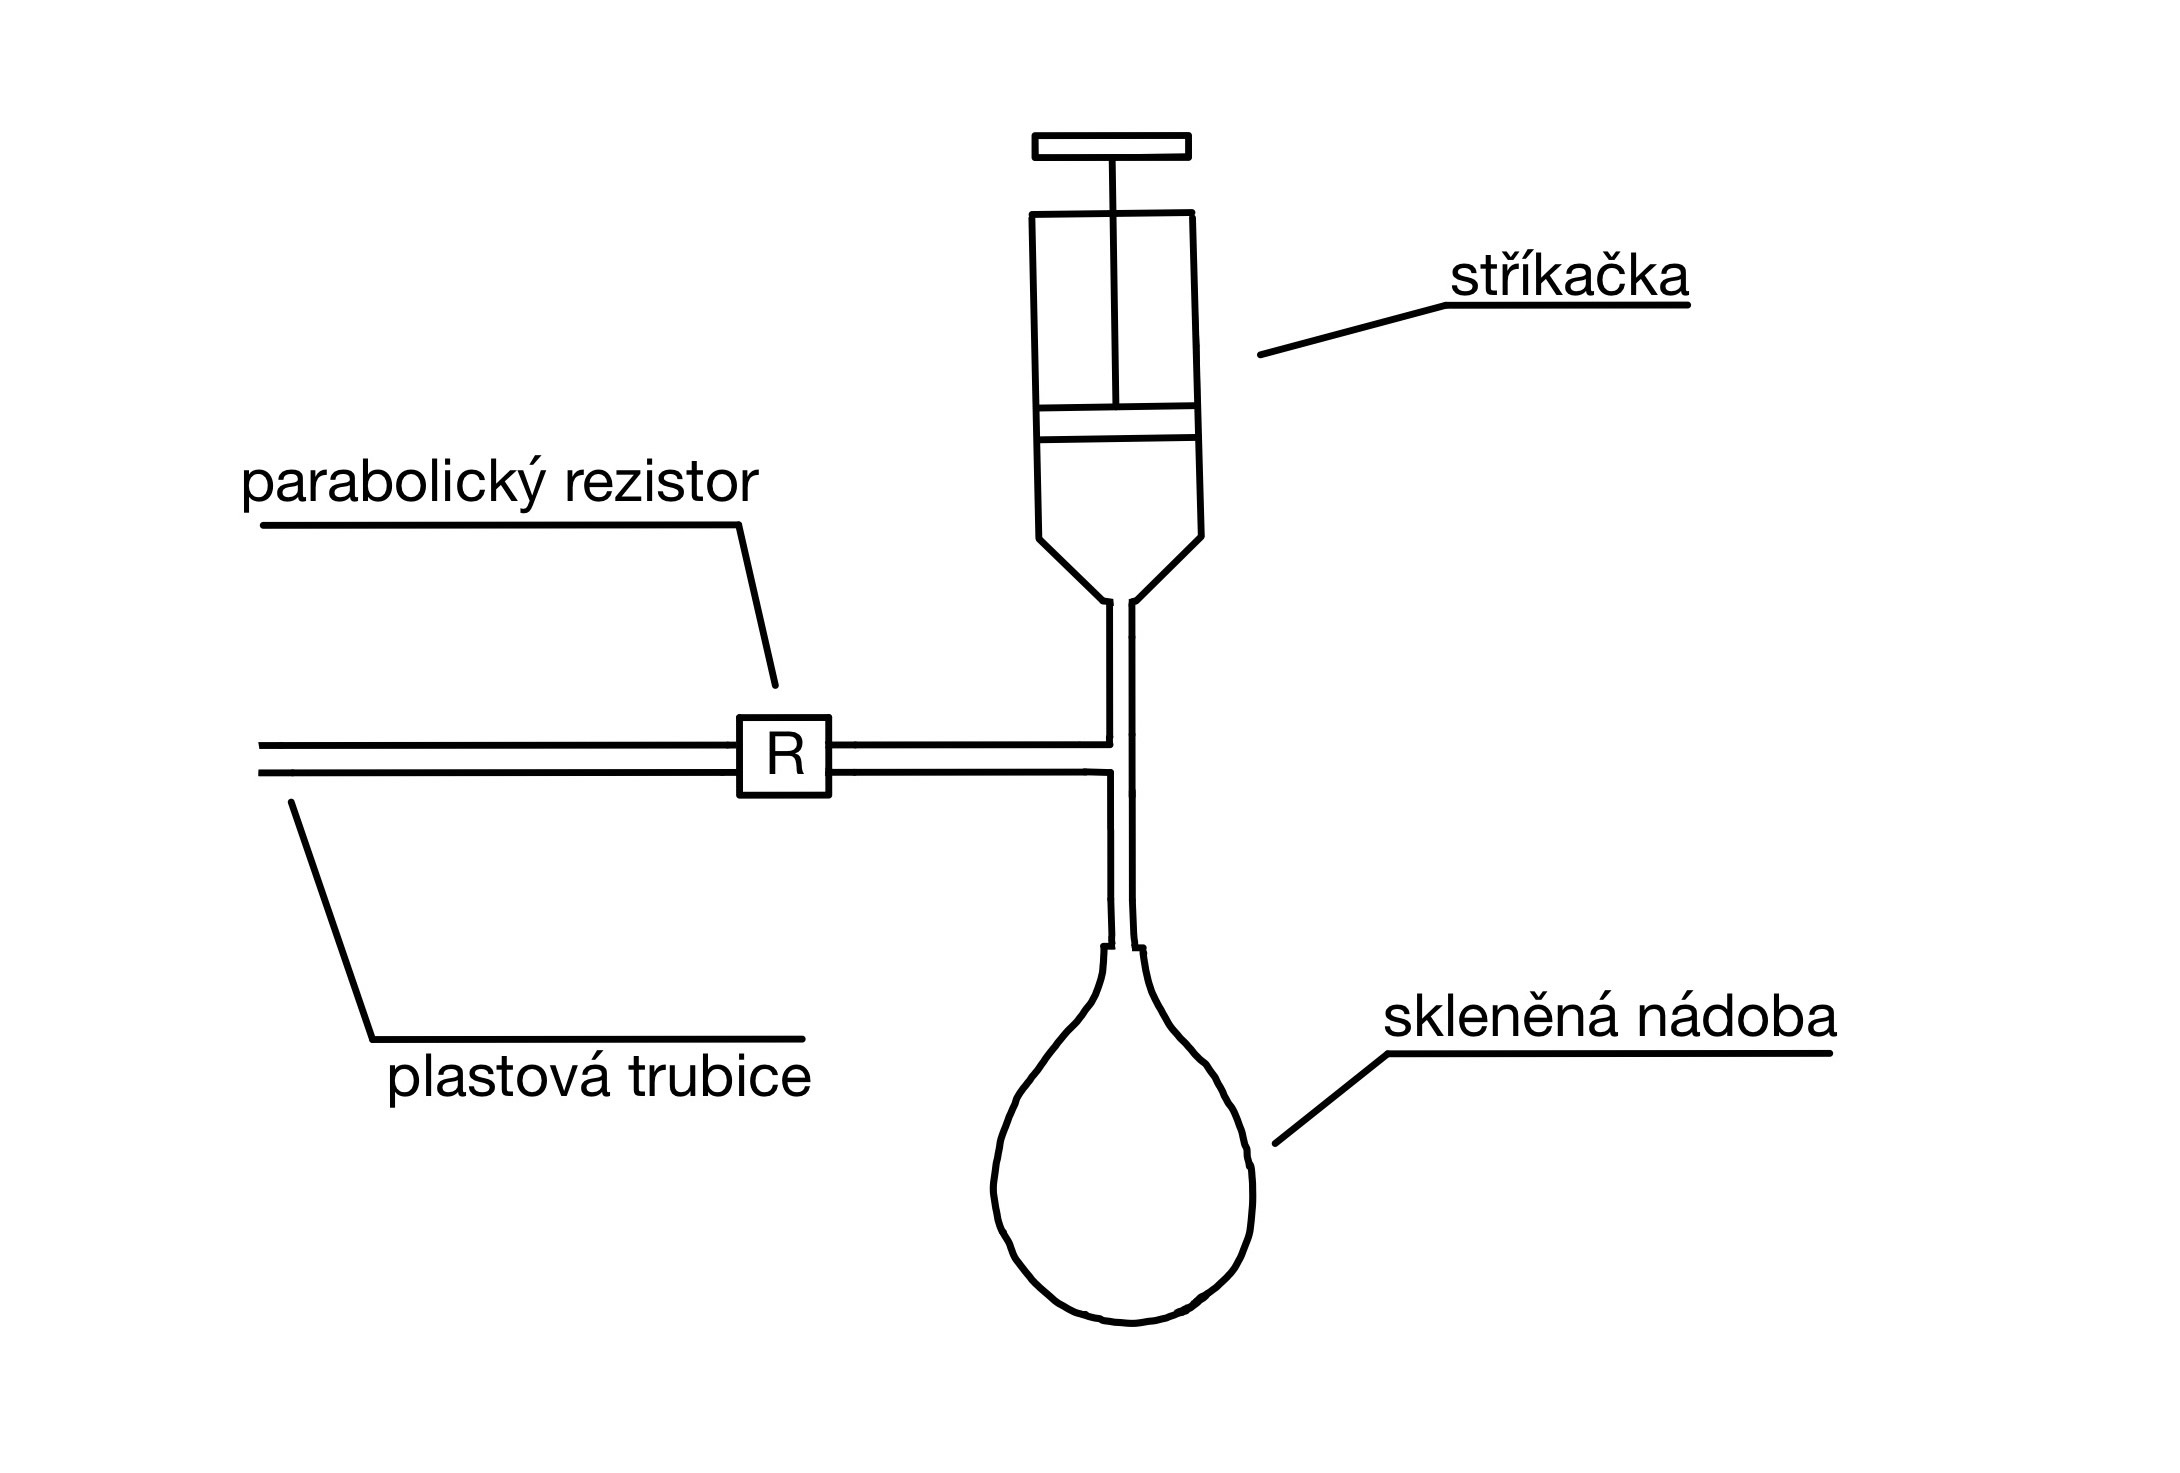
\includegraphics[width=1\textwidth]{schema}
			\caption{Schéma modelu respiračního systému}
			 \label{obrazekschema}
 \end{figure}

\begin{figure}[!ht]
			\centering
 			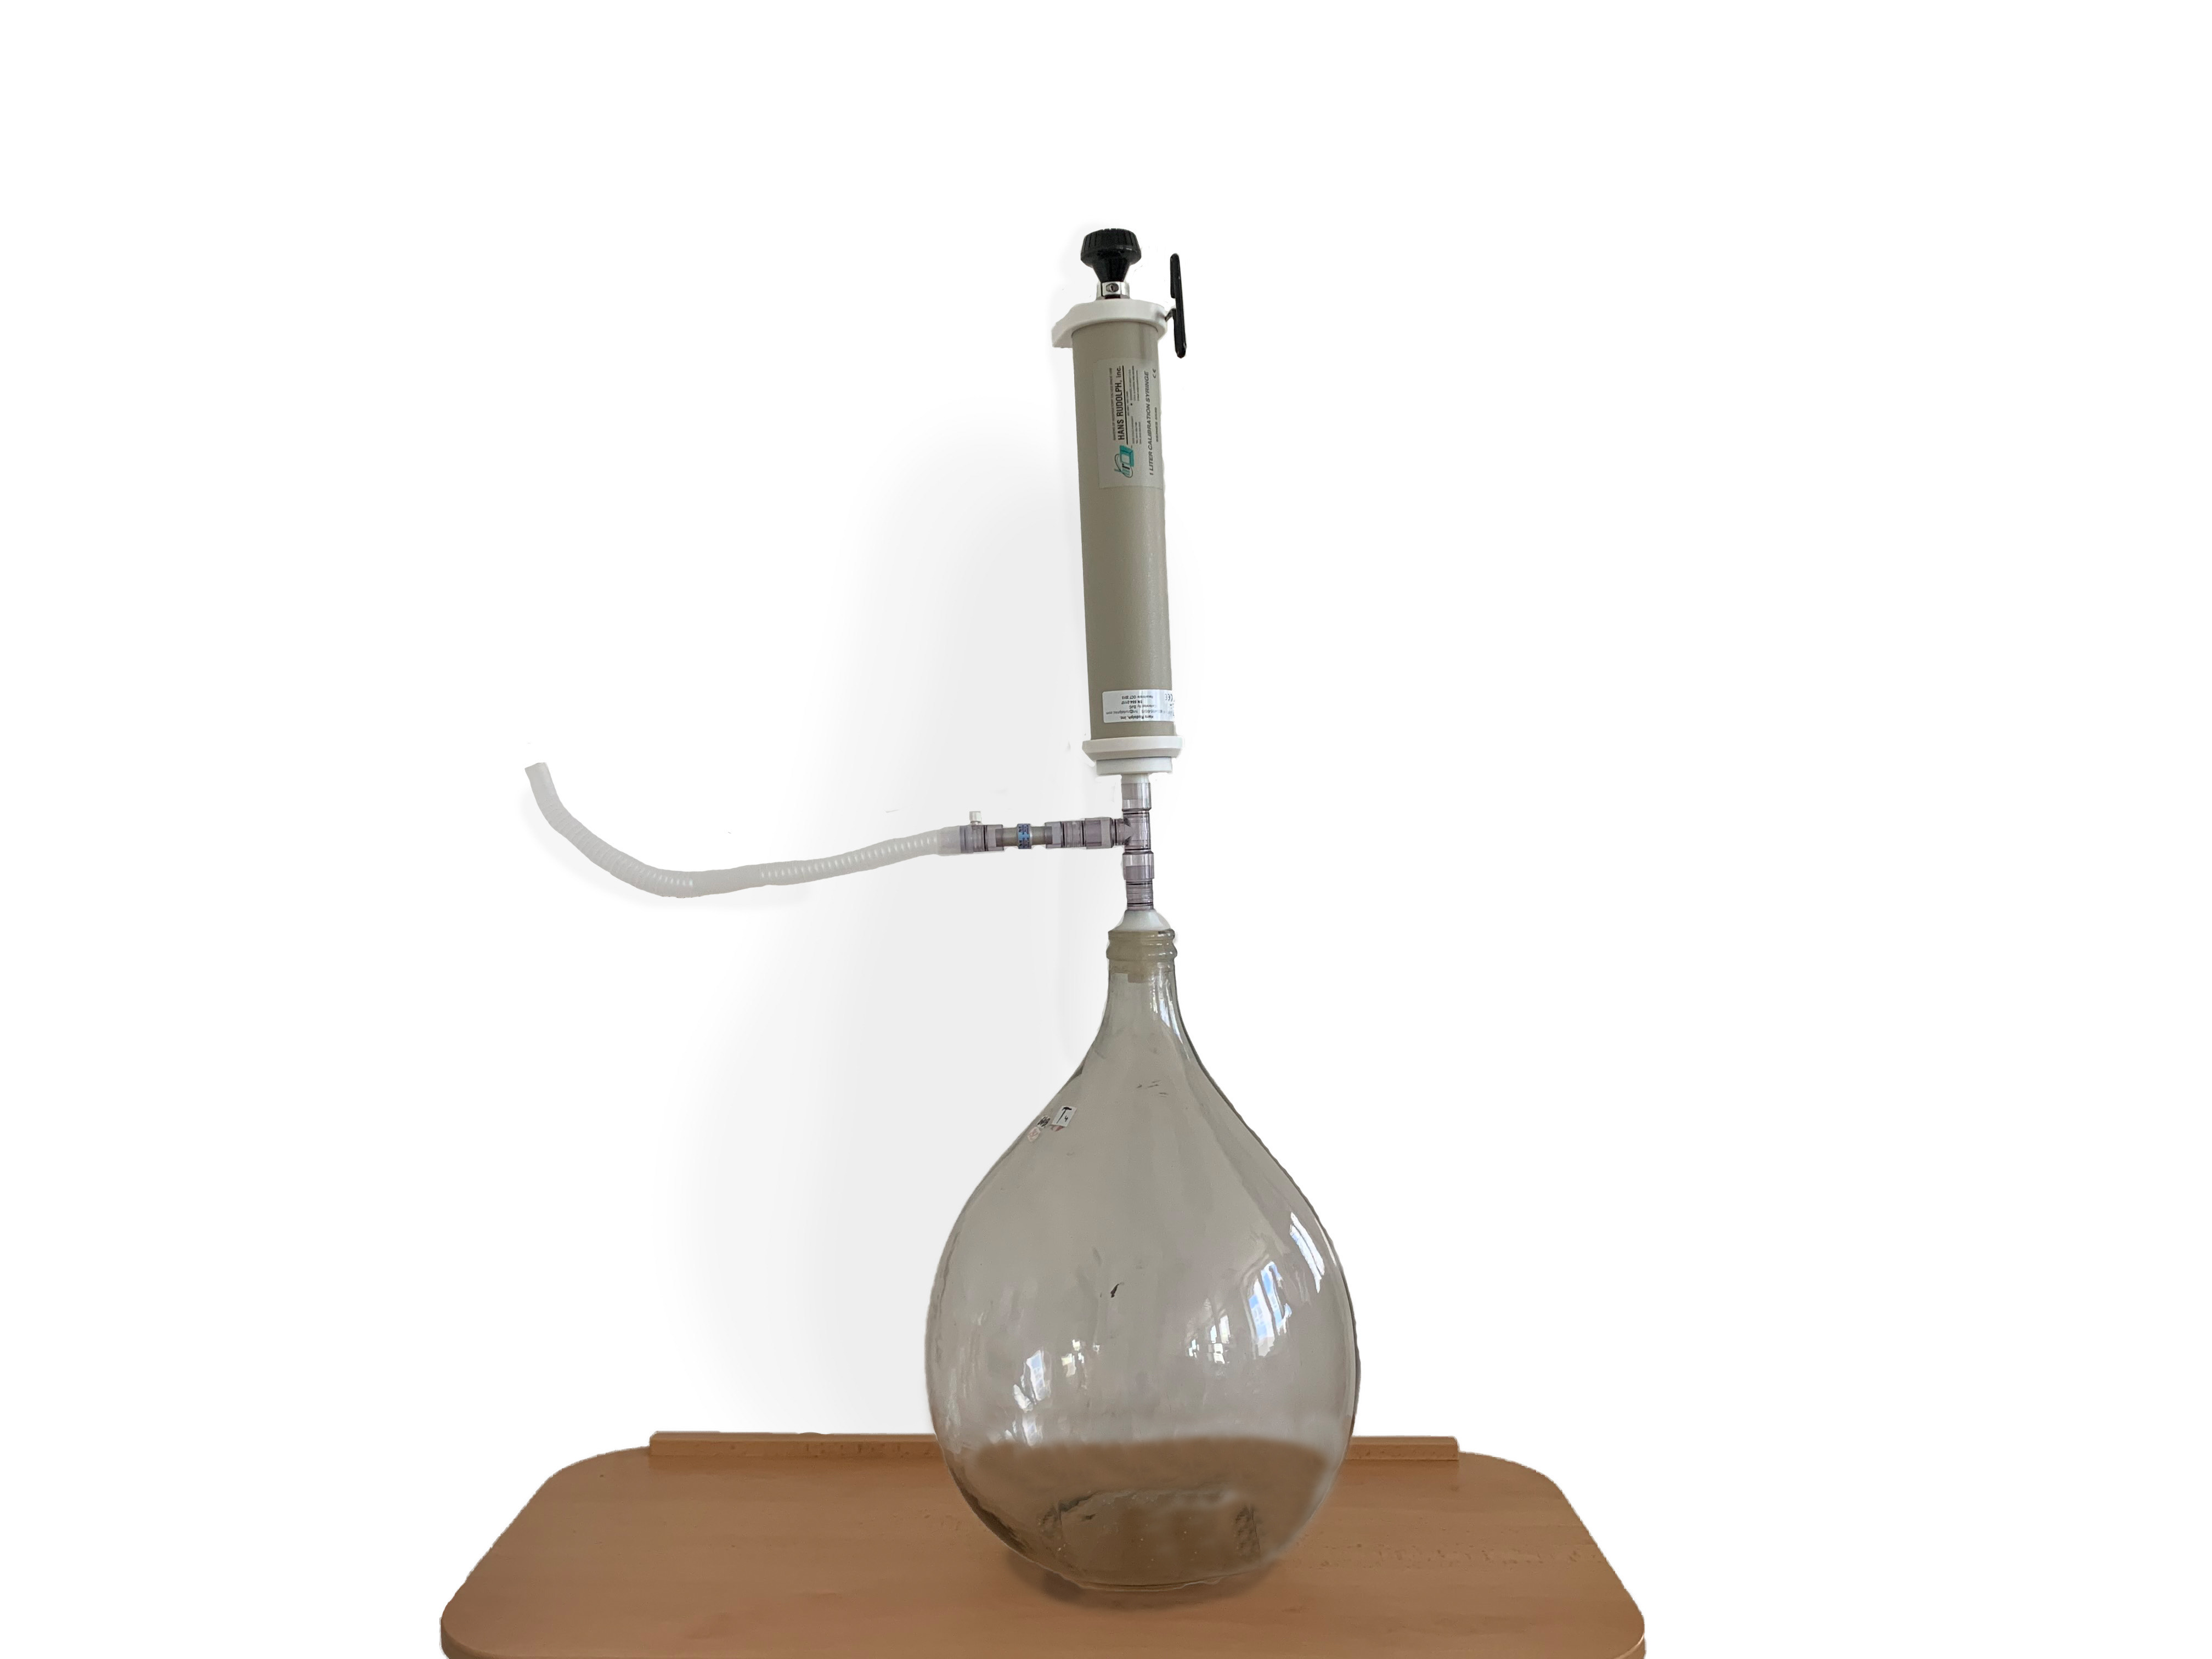
\includegraphics[width=1\textwidth]{fotka}
			\caption{Obrázek skutečného modelu respiračního systému}
			 \label{obrazekreal}
 \end{figure}

\clearpage

\subsection{Průběh měření}
Měření bylo prováděno v laboratoři pomocí přístroje tremoflo C-100 od firmy Thorasys. K měření byl třeba počítač s nainstalovaným softwarem pro tento přístroj. Na software tremoflo je třeba mít licenci, tudíž měření bylo možné provádět pouze na konkrétním počítači, kde je licence nainstalována.  Nejprve se přístroj i počítač zapojil do elektrické sítě a zapnul. Přístroj tremoflo C-100 se propojí s počítačem pomocí USB kabelu a po startu ovládacího software je potřeba provést kalibraci pomocí kalibrační zátěže, popis kalibrace je v podkapitole \ref{kalibrace}. Software nemá testovací režim, tudíž před měřením je třeba vytvořit kartu fiktivního pacienta. Do ní je třeba vyplnit  jméno, příjmení a věk pacienta. Po sestavení první kombinace modelu a vytvoření fiktivního pacienta se může přejít k měření. Každé měření probíhalo  \SI{16}{s} během kterých byla mechanicky stlačována střička, která do systému vháněla vzduch. Po  \SI{16}{s} přístroj data uložil a měření se opakovalo 3x kvůli snížení chyb a následnému průměrování. Po 3~měřeních jedné kombinace se jedna komponenta modelu, průtočný odpor, délka plastové trubice nebo velikost skleněné nádoby vyměnila a měření se opakovalo. Tímhle způsobem se vystřídaly všechny kombinace. Všechna data byla uložena v systému a potom se z~nich vygenerovala tabulka


	\clearpage
	
	\section{Výsledky}
	\label{kap-vysledky}
Laboratorní měření bylo provedeno celkem na 18~kombinacích modelu respiračního systému. Postupně byly vyměněny dvě velikosti nádob, 3 délky plastové trubice a 3 velikosti parabolického odporu. Přístroj měří několik veličin: reaktanci, rezistenci, objem, rezonanční frekvenci a $COH_{3}$. Tato práce popisuje změnu rezistance a reaktance s~ohledem na změnu různých komponent.  

 
\subsection{Rezistance}

Výsledky pro menší nádobu tj. \SI{35}{L} vyšly ve většině případů s menší odchylkou než výsledky měření s 54~litrovou nádobou. Pro odpor 20 vyšla rezistence cca o $\SI{0,5}{cm\cdot H_{2}O \cdot s/L} $větší u nádoby \SI{35}{L}. Hodnoty rezistence pro odpor 5 vyšly naopak vyšší pro nádobu s menším objemem. 

Pří měření s delší plastovou trubicí vyšly také výsledky s menší odchylkou. 
Při zvětšení inertance, neboli použití delší plastové trubice se rezistence u~všech velikostí průtočného odporu cca o  $\SI{0,5}{ cm\cdot H_{2}O \cdot s/L} $ zvýší. 
Při zvýšení poddajnosti, tj. při použití nádoby s  větším objemem rezistence o cca  $\SI{0,5}{ cm\cdot H_{2}O \cdot s/L} $  klesne. 
Při použití Rp~20 je rezistence o také cca  $\SI{0,5}{ cm\cdot H_{2}O \cdot s/L} $  vyšší než u Rp~5 a Rp~50. 

\subsection{Reaktance}

Čím víc se snižovala inertance, tj. čím kratší byla plastová trubice tím víc klesala i reaktance. Při větší poddajnosti se reaktance zvedla. Stejně jako u rezistence byla i reaktance nejvyšší při použití Rp~20. Odchylky pro měření s větší i menší nádobou jsou podobné. 


Měřena byla především rezistence, reaktance, rezonanční frekvence, objem a $COH_{3}$. 



\begin{figure}
\centering
\begin{minipage}{.5\textwidth}
  \centering
  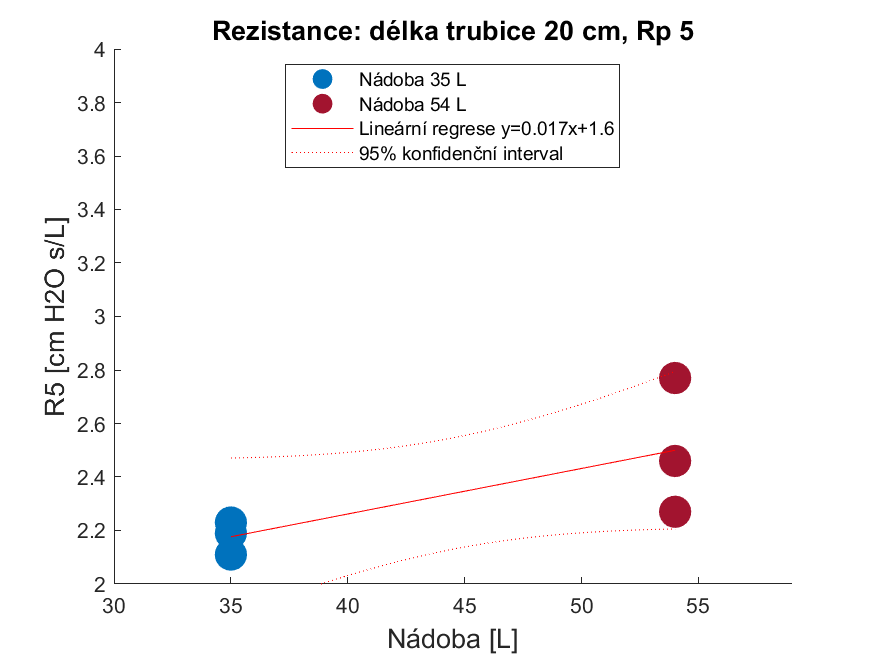
\includegraphics[width=1\linewidth]{rezistance_dily_20_odpor_5}
\captionsetup{justification=centering}
  \captionof{figure}{Rezistance: délka~trubice~$\SI{20}{cm}$, Rp~$\SI{5}{}$}
\end{minipage}%
\begin{minipage}{.5\textwidth}
  \centering
  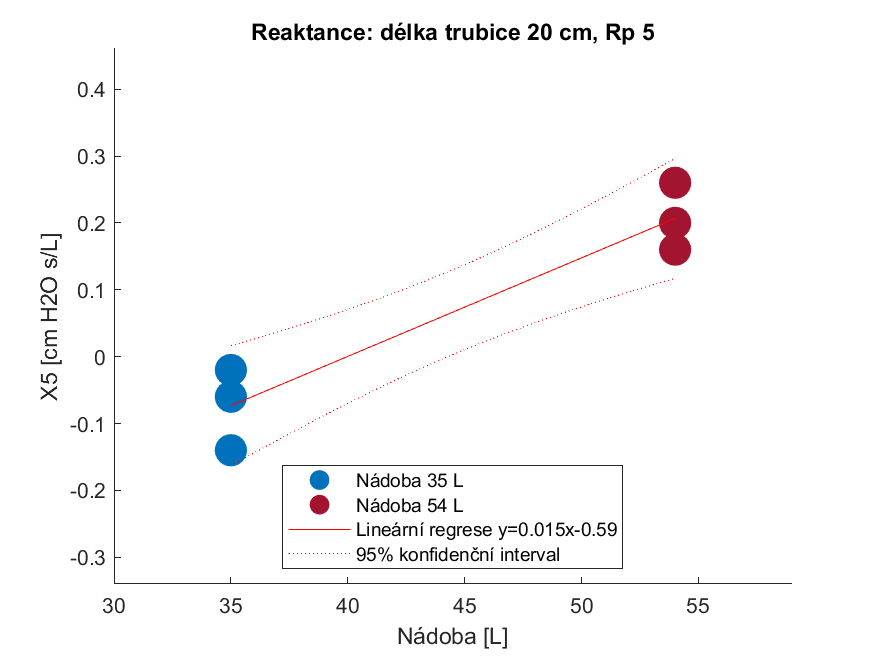
\includegraphics[width=1\linewidth]{reaktance_dily_20_odpor_5}
\captionsetup{justification=centering}
  \captionof{figure}{Reaktance: délka~trubice~$\SI{20}{cm}$, Rp~$\SI{5}{}$}
\end{minipage}
\end{figure}


\begin{figure}
\centering
\begin{minipage}{.5\textwidth}
  \centering
  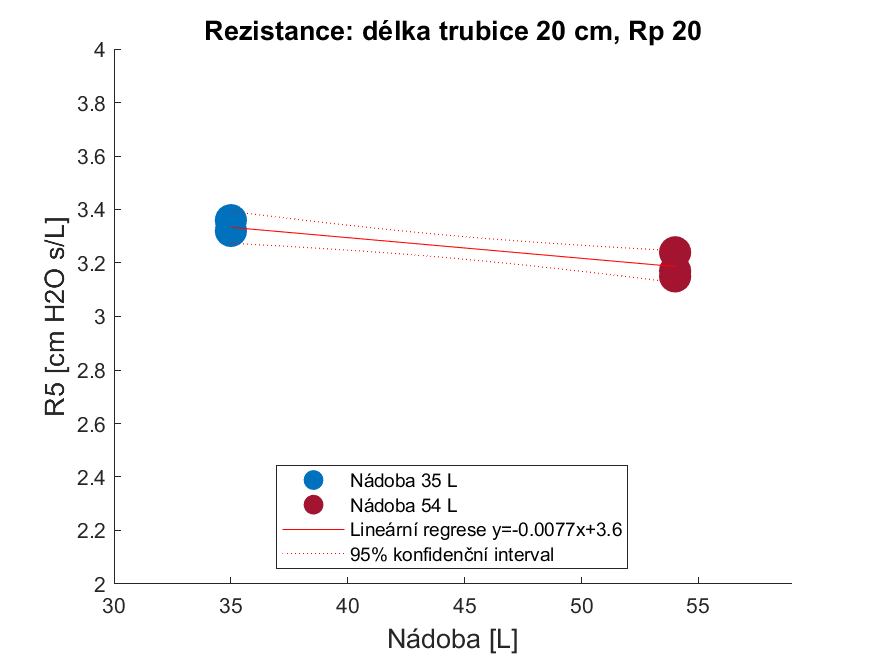
\includegraphics[width=1\linewidth]{rezistance_dily_20_odpor_20}
\captionsetup{justification=centering}
  \captionof{figure}{Rezistance: délka~trubice~$\SI{20}{cm}$, Rp~$\SI{20}{}$}
 \label{rezistance-dily-20-odpor-20}
\end{minipage}%
\begin{minipage}{.5\textwidth}
  \centering
  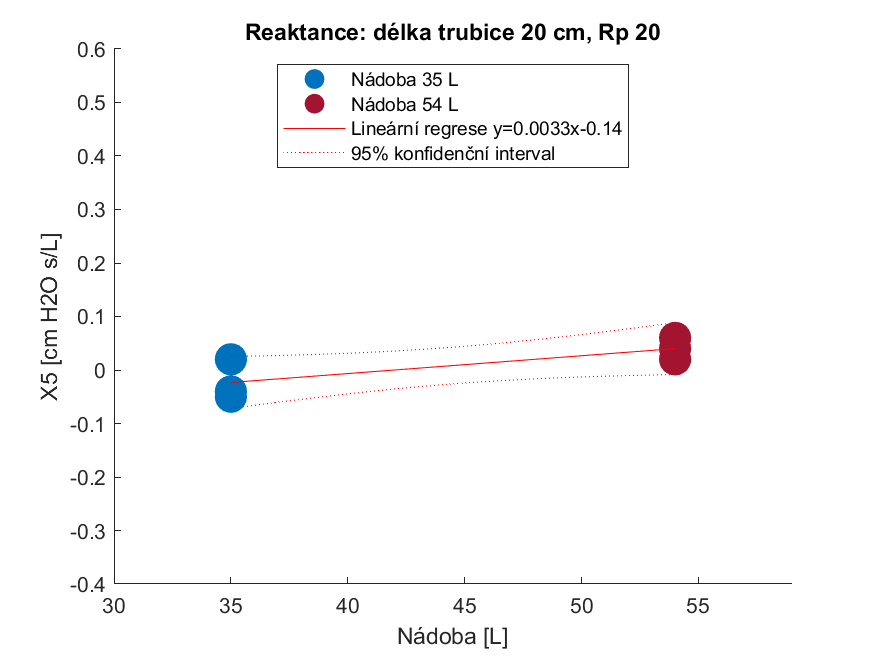
\includegraphics[width=1\linewidth]{reaktance_dily_20_odpor_20}
\captionsetup{justification=centering}
  \captionof{figure}{Reaktance: délka~trubice~$\SI{20}{cm}$, Rp~$\SI{20}{}$}
\end{minipage}
\end{figure}

\begin{figure}
\centering
\begin{minipage}{.5\textwidth}
  \centering
  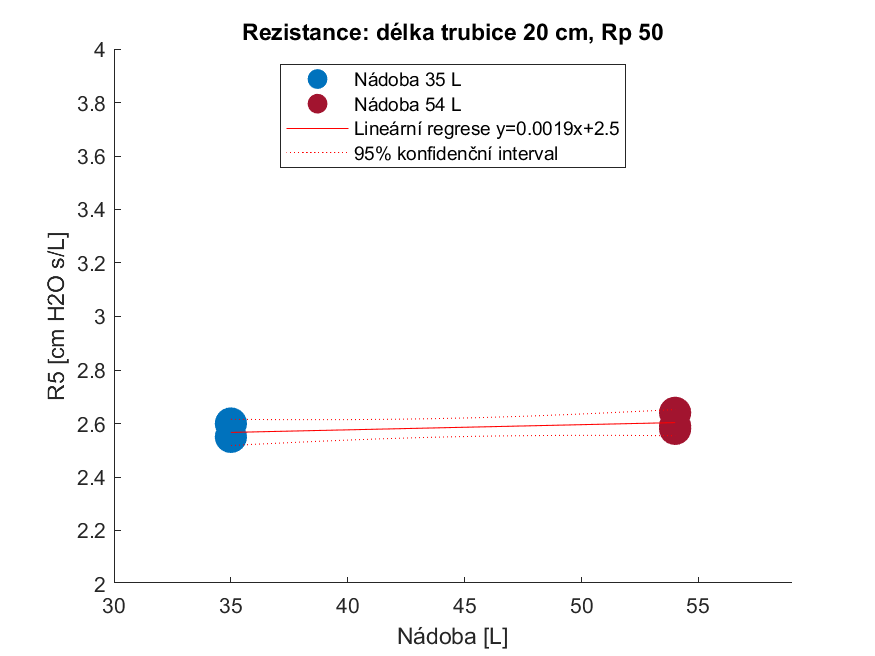
\includegraphics[width=1\linewidth]{rezistance_dily_20_odpor_50}
\captionsetup{justification=centering}
  \captionof{figure}{Rezistance: délka~trubice~$\SI{20}{cm}$, Rp~$\SI{50}{}$}
\end{minipage}%
\begin{minipage}{.5\textwidth}
  \centering
  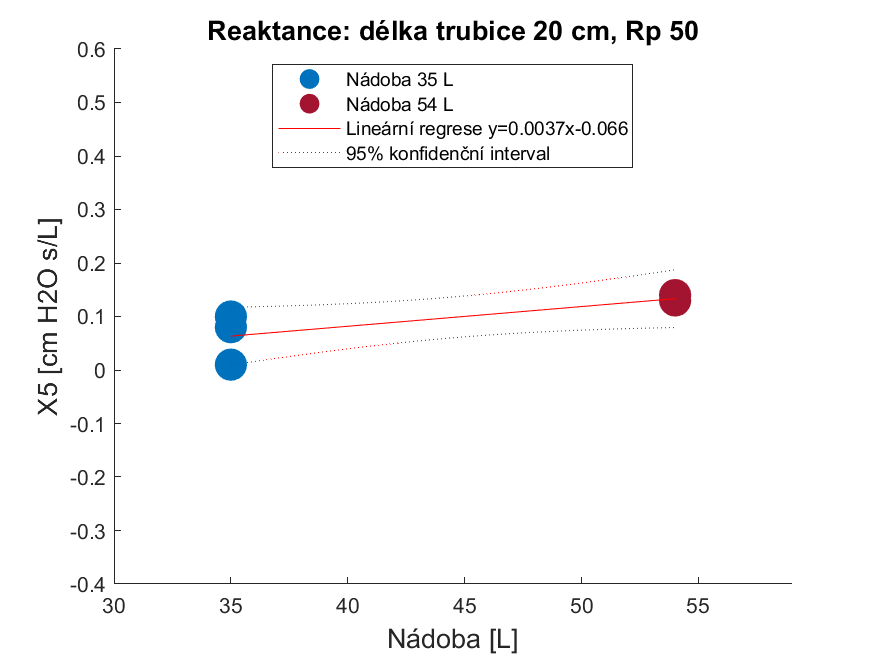
\includegraphics[width=1\linewidth]{reaktance_dily_20_odpor_50}
\captionsetup{justification=centering}
  \captionof{figure}{Reaktance: délka~trubice~$\SI{20}{cm}$, Rp~$\SI{50}{}$}
\end{minipage}
\end{figure}



\begin{figure}
\centering
\begin{minipage}{.5\textwidth}
  \centering
  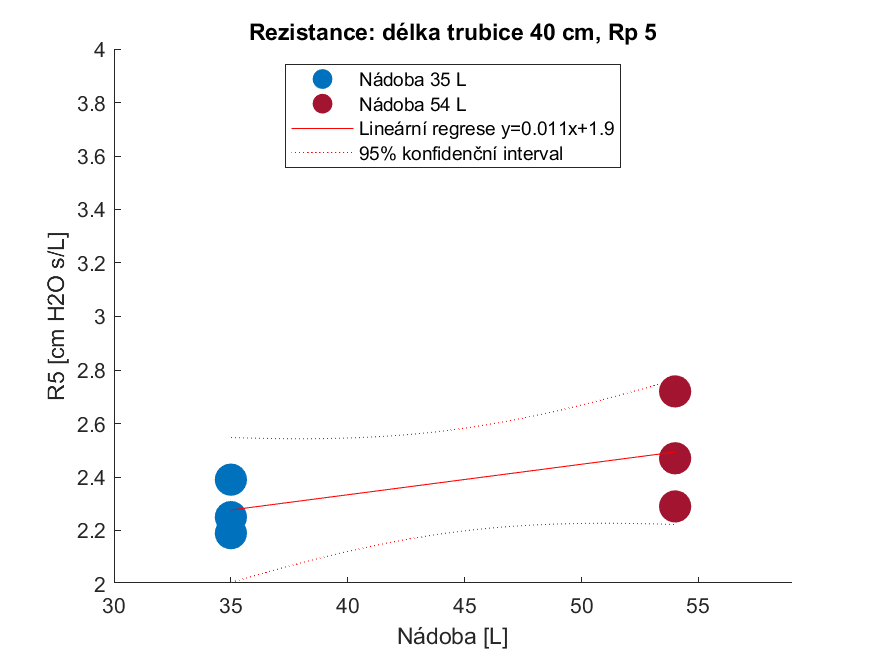
\includegraphics[width=1\linewidth]{rezistance_dily_40_odpor_5}
\captionsetup{justification=centering}
  \captionof{figure}{Rezistance: délka~trubice~$\SI{40}{cm}$, Rp~$\SI{5}{}$}
\label{rezistance_dily_40_odpor_5}
\end{minipage}%
\begin{minipage}{.5\textwidth}
  \centering
  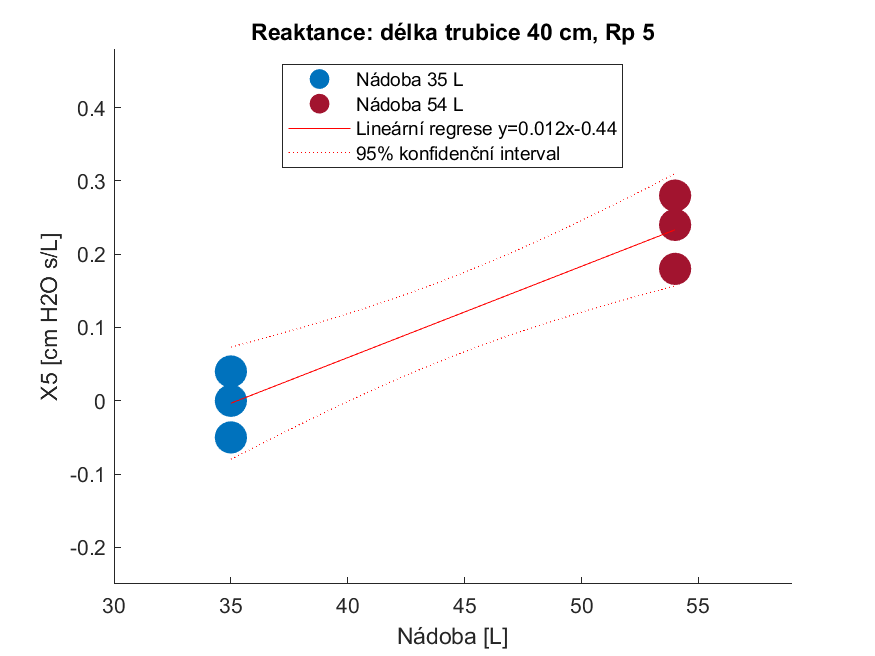
\includegraphics[width=1\linewidth]{reaktance_dily_40_odpor_5}
\captionsetup{justification=centering}
  \captionof{figure}{Reaktance: délka~trubice~$\SI{40}{cm}$, Rp~$\SI{5}{}$}
\end{minipage}
\end{figure}

\begin{figure}
\centering
\begin{minipage}{.5\textwidth}
  \centering
  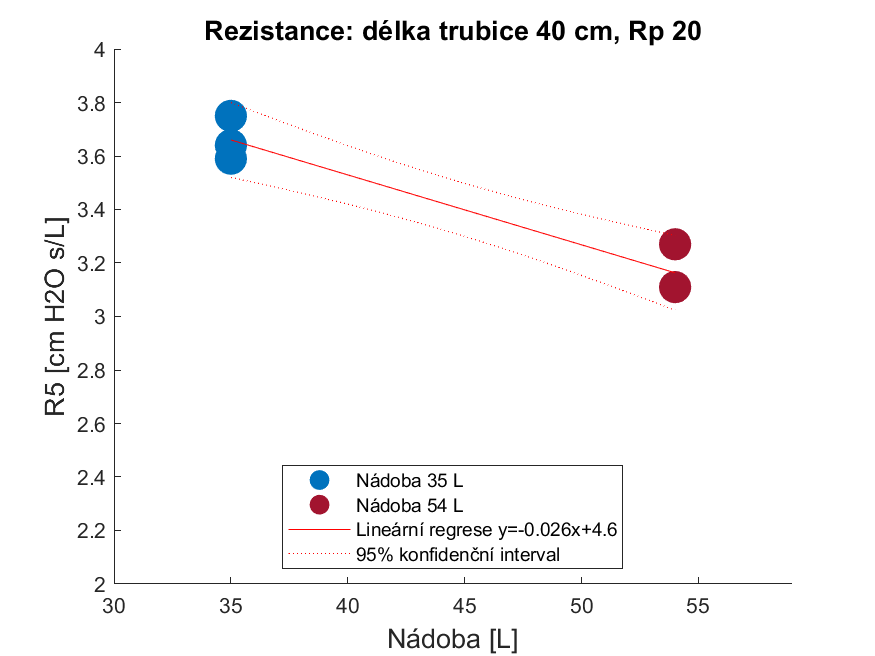
\includegraphics[width=1\linewidth]{rezistance_dily_40_odpor_20}
\captionsetup{justification=centering}
  \captionof{figure}{Rezistance: délka~trubice~$\SI{40}{cm}$, Rp~$\SI{20}{}$}
\label{rezistance_dily_40_odpor_20}
\end{minipage}%
\begin{minipage}{.5\textwidth}
  \centering
  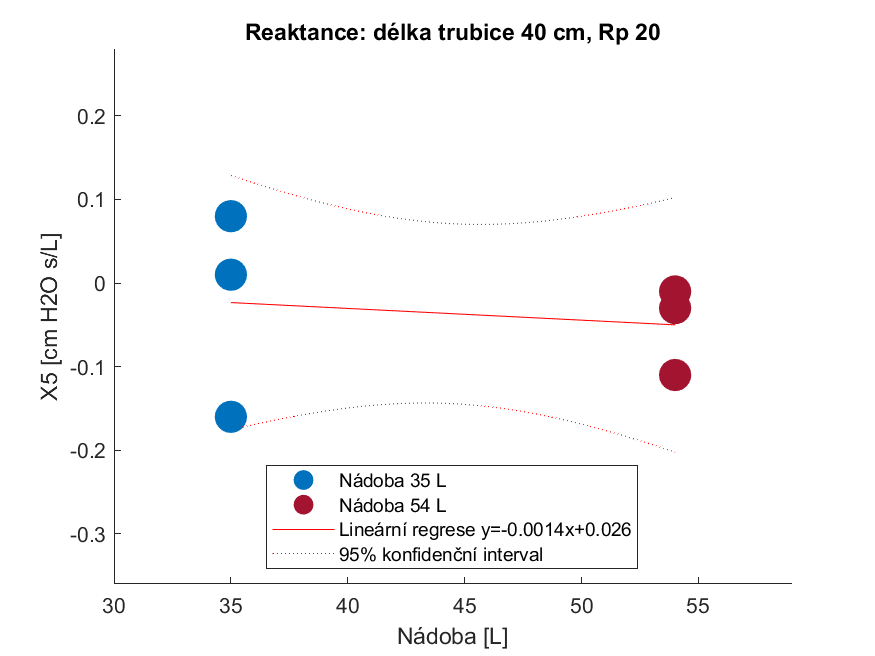
\includegraphics[width=1\linewidth]{reaktance_dily_40_odpor_20}
\captionsetup{justification=centering}
  \captionof{figure}{Reaktance: délka~trubice~$\SI{40}{cm}$, Rp~$\SI{20}{}$}
\end{minipage}
\end{figure}

\begin{figure}
\centering
\begin{minipage}{.5\textwidth}
  \centering
  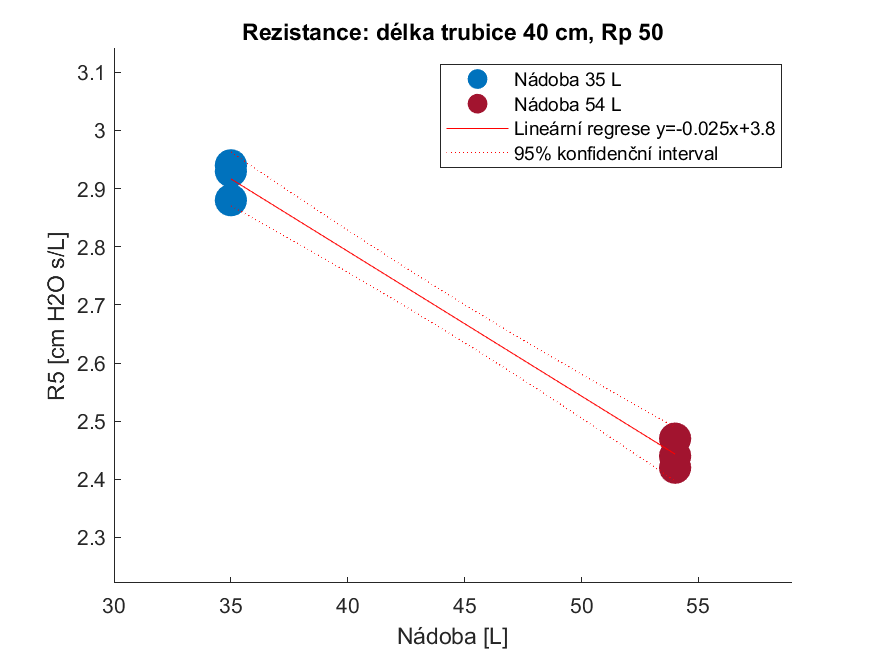
\includegraphics[width=1\linewidth]{rezistance_dily_40_odpor_50}
\captionsetup{justification=centering}
  \captionof{figure}{Rezistance: délka~trubice~$\SI{40}{cm}$, Rp~$\SI{50}{}$}
\label{rezistance_dily_40_odpor_50}
\end{minipage}%
\begin{minipage}{.5\textwidth}
  \centering
  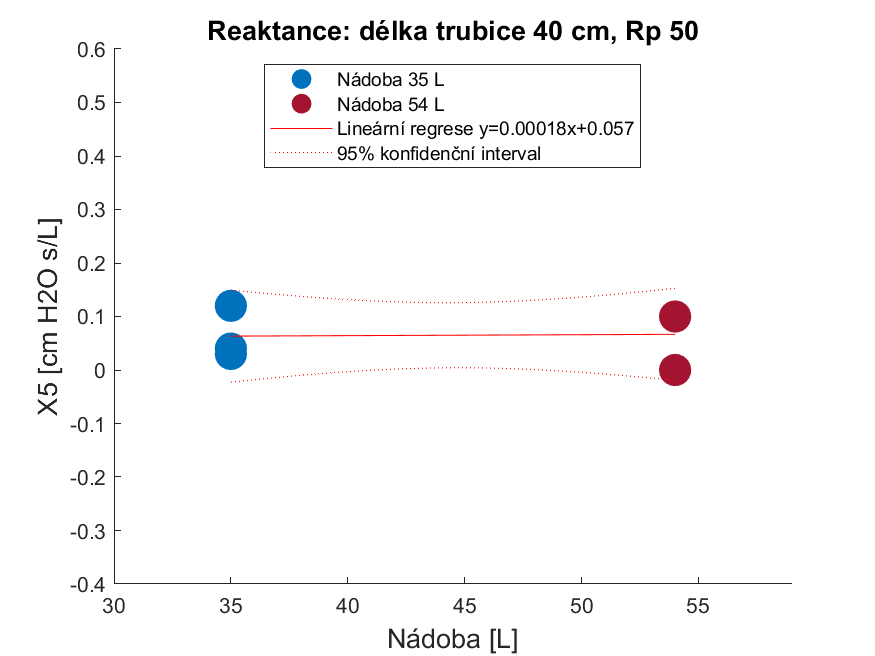
\includegraphics[width=1\linewidth]{reaktance_dily_40_odpor_50}
\captionsetup{justification=centering}
  \captionof{figure}{Reaktance: délka~trubice~$\SI{40}{cm}$, Rp~$\SI{50}{}$}
\end{minipage}
\end{figure}





\begin{figure}
\centering
\begin{minipage}{.5\textwidth}
  \centering
  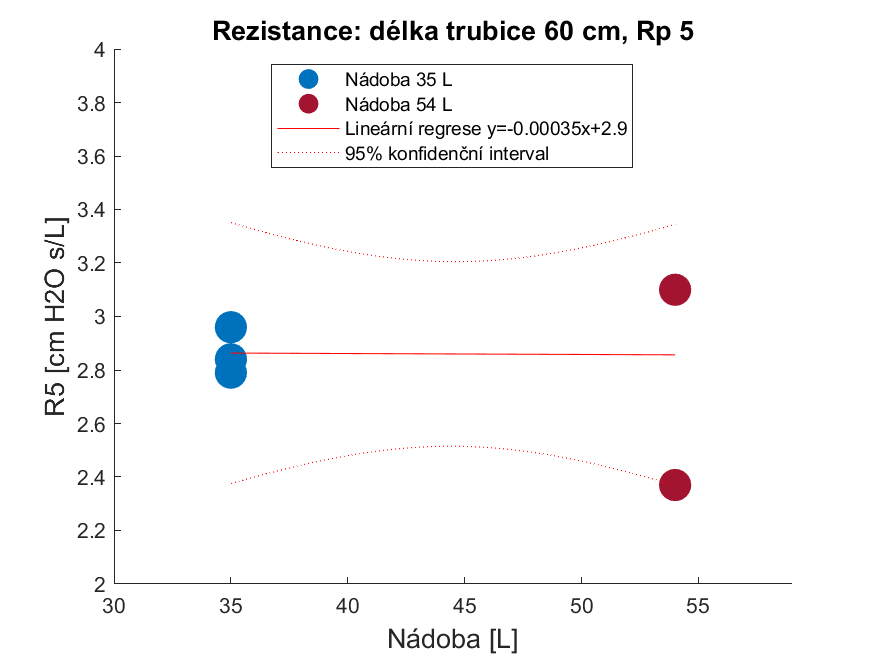
\includegraphics[width=1\linewidth]{rezistance_dily_60_odpor_5}
\captionsetup{justification=centering}
  \captionof{figure}{Rezistance: délka~trubice~$\SI{60}{cm}$, Rp~$\SI{5}{}$}
\end{minipage}%
\begin{minipage}{.5\textwidth}
  \centering
  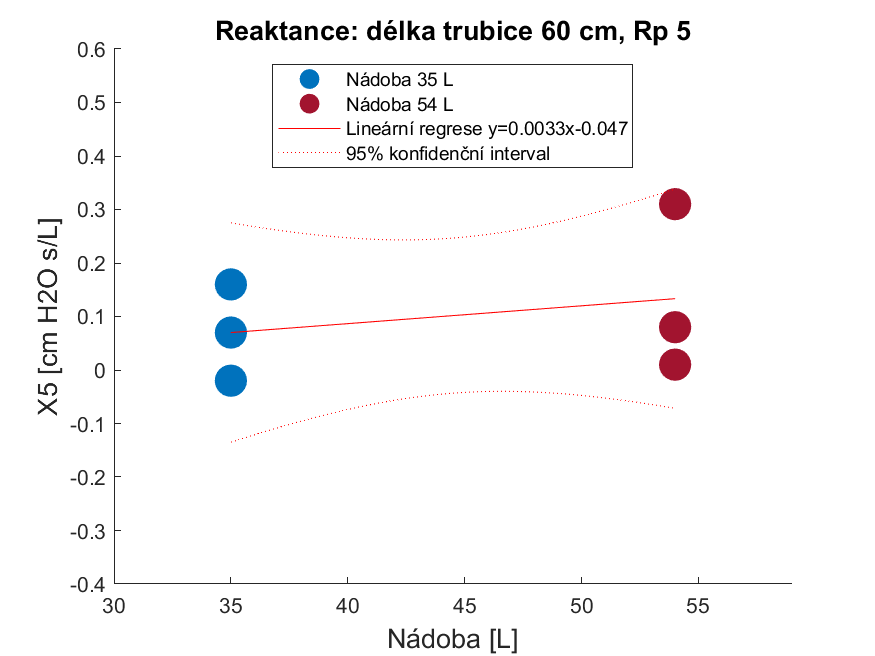
\includegraphics[width=1\linewidth]{reaktance_dily_60_odpor_5}
\captionsetup{justification=centering}
  \captionof{figure}{Reaktance: délka~trubice~$\SI{60}{cm}$, Rp~$\SI{5}{}$}
\end{minipage}
\end{figure}

\begin{figure}
\centering
\begin{minipage}{.5\textwidth}
  \centering
  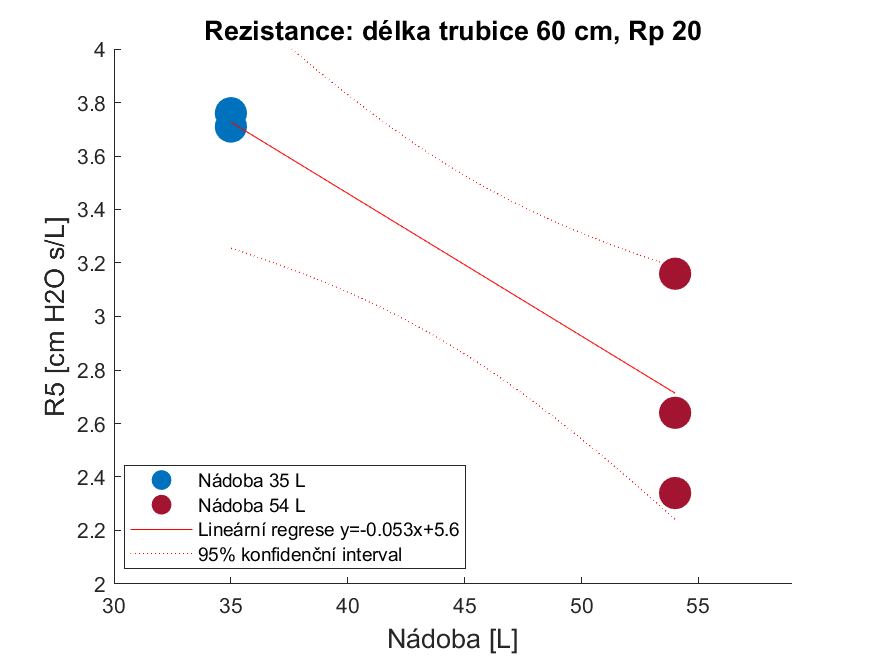
\includegraphics[width=1\linewidth]{rezistance_dily_60_odpor_20}
\captionsetup{justification=centering}
  \captionof{figure}{Rezistance: délka~trubice~$\SI{60}{cm}$, Rp~$\SI{20}{}$}
\end{minipage}%
\begin{minipage}{.5\textwidth}
  \centering
  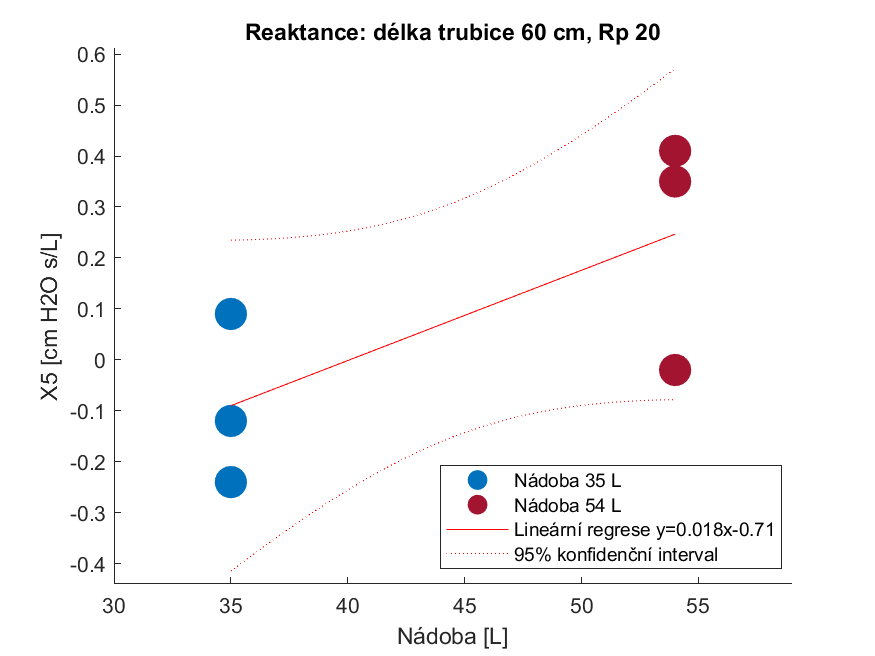
\includegraphics[width=1\linewidth]{reaktance_dily_60_odpor_20}
\captionsetup{justification=centering}
  \captionof{figure}{Reaktance: délka~trubice~$\SI{60}{cm}$, Rp~$\SI{20}{}$}
\end{minipage}
\end{figure}

\begin{figure}
\centering
\begin{minipage}{.5\textwidth}
  \centering
  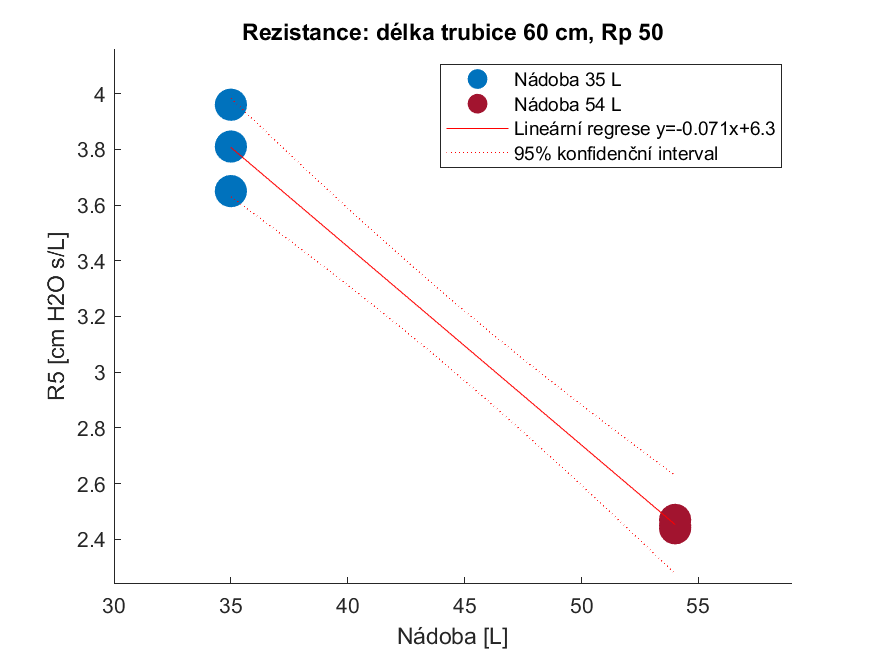
\includegraphics[width=1\linewidth]{rezistance_dily_60_odpor_50}
\captionsetup{justification=centering}
  \captionof{figure}{Rezistance: délka~trubice~$\SI{60}{cm}$, Rp~$\SI{50}{}$}
\end{minipage}%
\begin{minipage}{.5\textwidth}
  \centering
  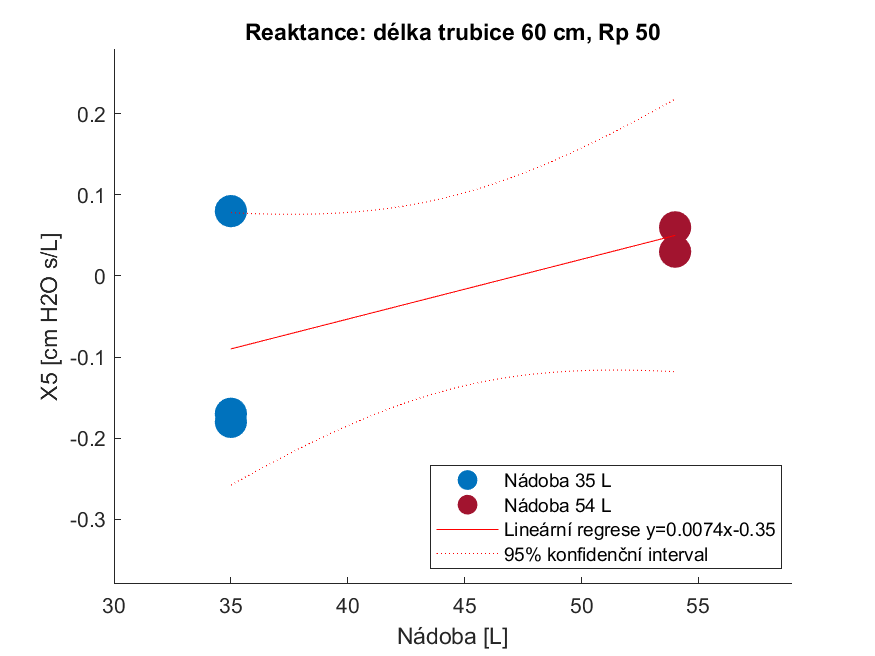
\includegraphics[width=1\linewidth]{reaktance_dily_60_odpor_50}
\captionsetup{justification=centering}
  \captionof{figure}{Reaktance: délka~trubice~$\SI{60}{cm}$, Rp~$\SI{50}{}$}
\end{minipage}
\end{figure}




\begin{figure}
\centering
\begin{minipage}{.5\textwidth}
  \centering
  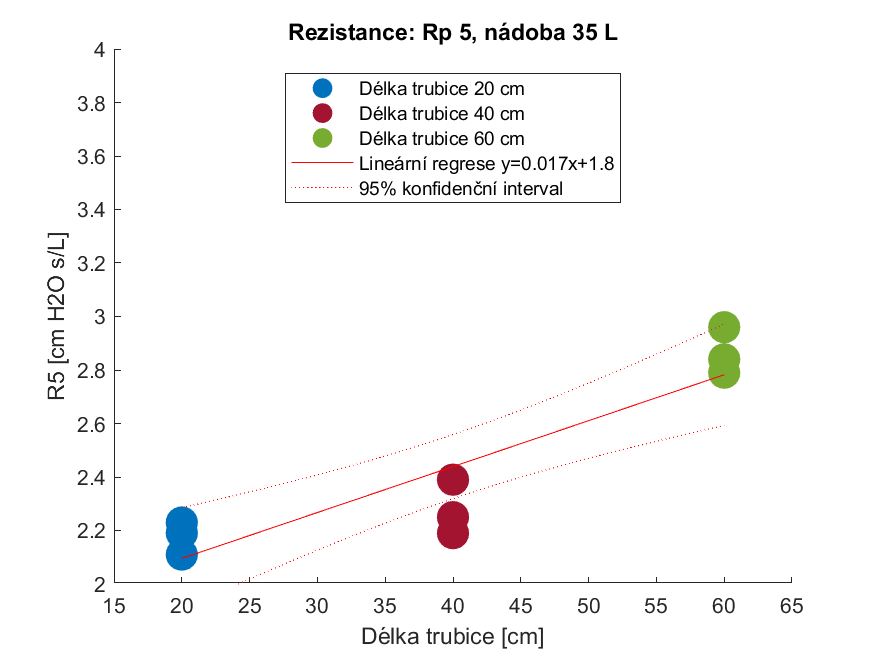
\includegraphics[width=1\linewidth]{rezistance_odpor_5_nadoba_35}
\captionsetup{justification=centering}
  \captionof{figure}{Rezistance: Rp~$\SI{5}{}$,~nádoba~$\SI{35}{L}$}
\end{minipage}%
\begin{minipage}{.5\textwidth}
  \centering
  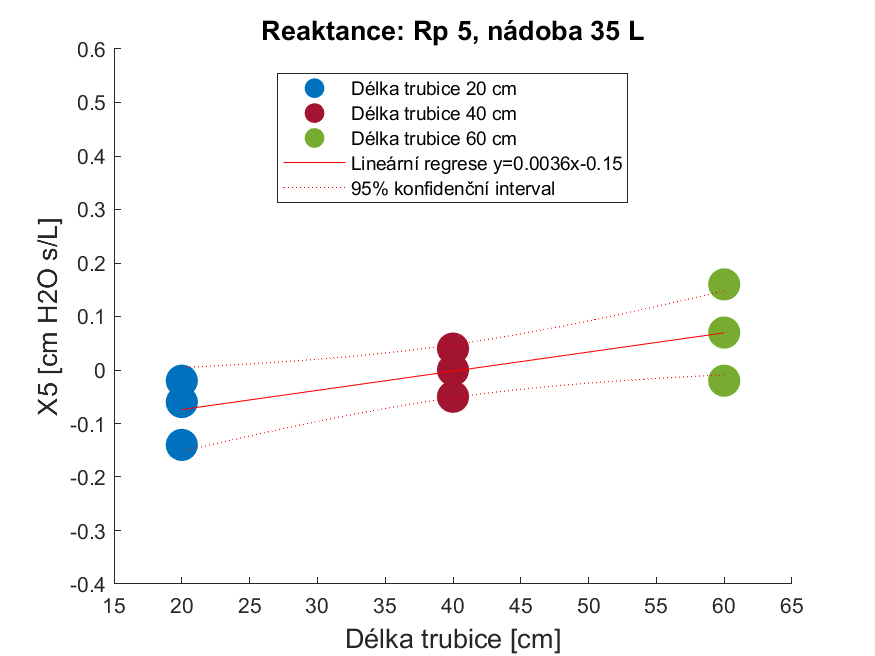
\includegraphics[width=1\linewidth]{reaktance_odpor_5_nadoba_35}
\captionsetup{justification=centering}
   \captionof{figure}{Reaktance: Rp~$\SI{5}{}$,~nádoba~$\SI{35}{L}$}
\end{minipage}
\end{figure}

\begin{figure}
\centering
\begin{minipage}{.5\textwidth}
  \centering
  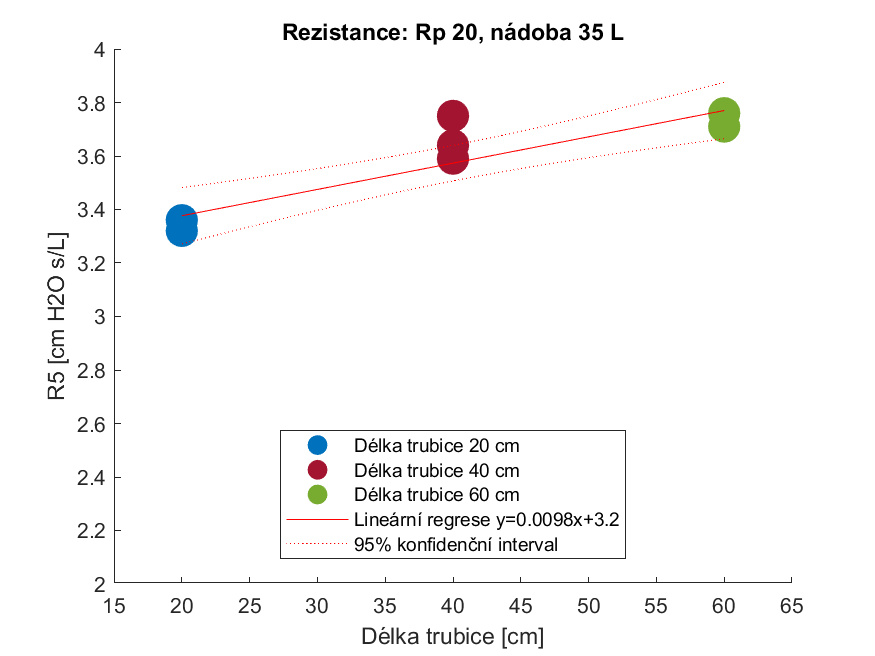
\includegraphics[width=1\linewidth]{rezistance_odpor_20_nadoba_35}
\captionsetup{justification=centering}
  \captionof{figure}{Rezistance: Rp~$\SI{20}{}$,~nádoba~$\SI{35}{L}$}
\end{minipage}%
\begin{minipage}{.5\textwidth}
  \centering
  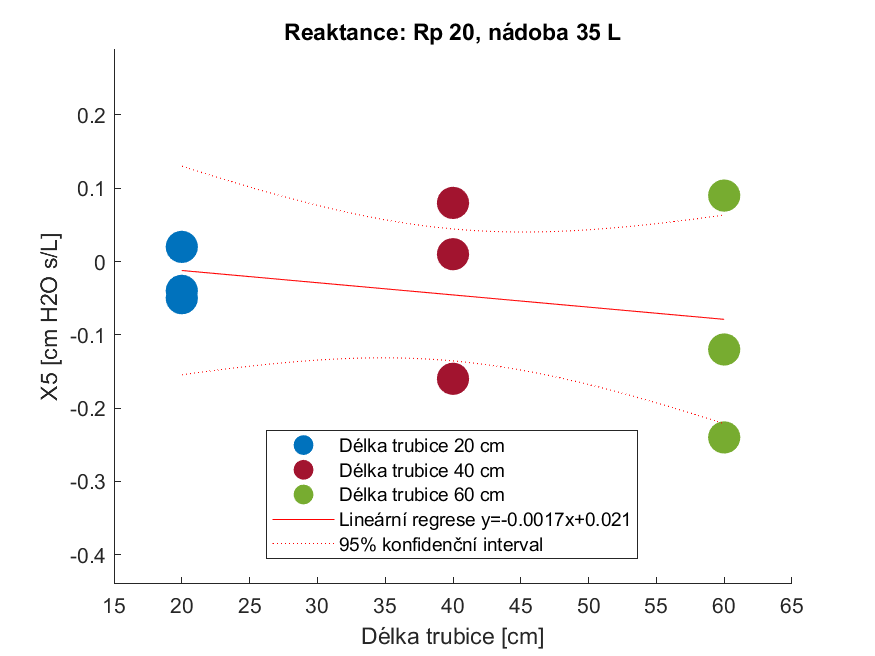
\includegraphics[width=1\linewidth]{reaktance_odpor_20_nadoba_35}
\captionsetup{justification=centering}
   \captionof{figure}{Reaktance: Rp~$\SI{20}{}$,~nádoba~$\SI{35}{L}$}
\end{minipage}
\end{figure}

\begin{figure}
\centering
\begin{minipage}{.5\textwidth}
  \centering
  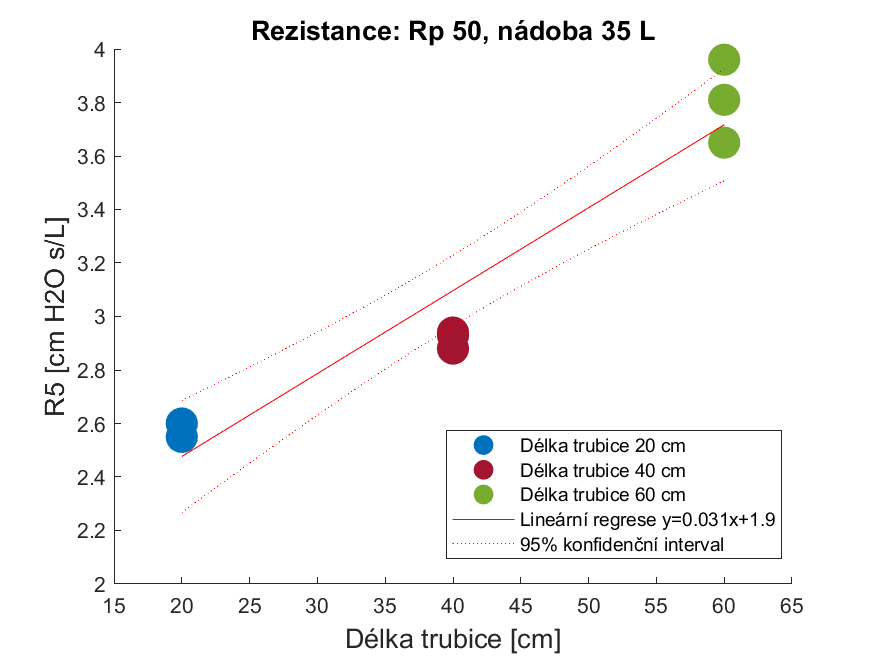
\includegraphics[width=1\linewidth]{rezistance_odpor_50_nadoba_35}
\captionsetup{justification=centering}
  \captionof{figure}{Rezistance: Rp~$\SI{50}{}$,~nádoba~$\SI{35}{L}$}
\end{minipage}%
\begin{minipage}{.5\textwidth}
  \centering
  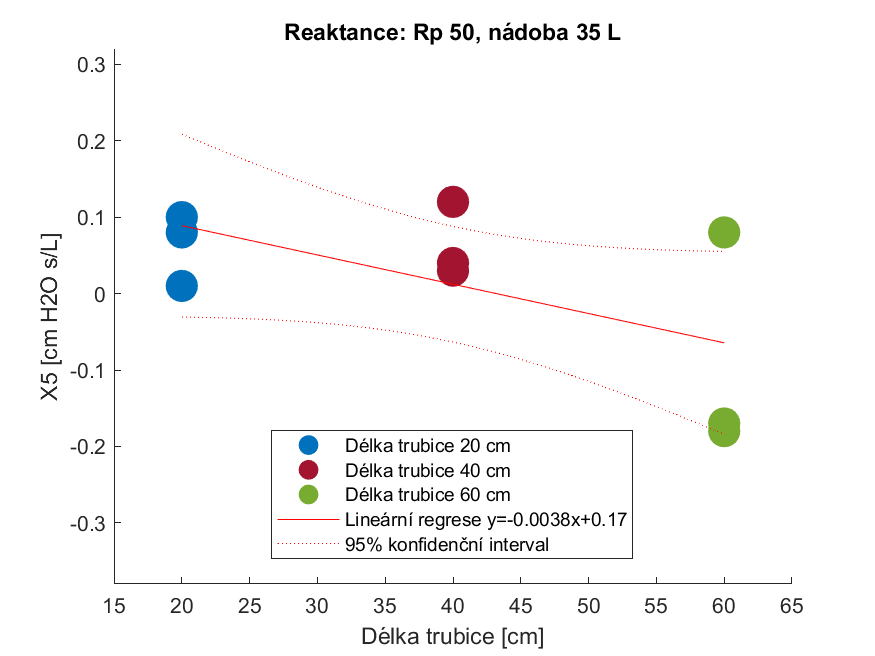
\includegraphics[width=1\linewidth]{reaktance_odpor_50_nadoba_35}
\captionsetup{justification=centering}
   \captionof{figure}{Reaktance: Rp~$\SI{50}{}$,~nádoba~$\SI{35}{L}$}
\end{minipage}
\end{figure}




\begin{figure}
\centering
\begin{minipage}{.5\textwidth}
  \centering
  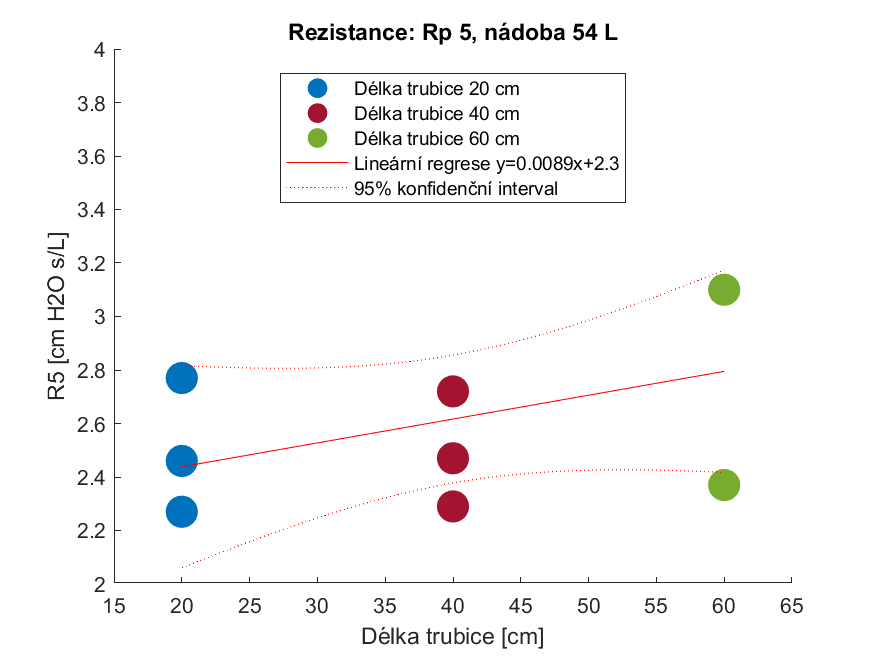
\includegraphics[width=1\linewidth]{rezistance_odpor_5_nadoba_54}
\captionsetup{justification=centering}
  \captionof{figure}{Rezistance: Rp~$\SI{5}{}$,~nádoba~$\SI{54}{L}$}
\label{rezistance_odpor_5_nadoba_54}
\end{minipage}%
\begin{minipage}{.5\textwidth}
  \centering
  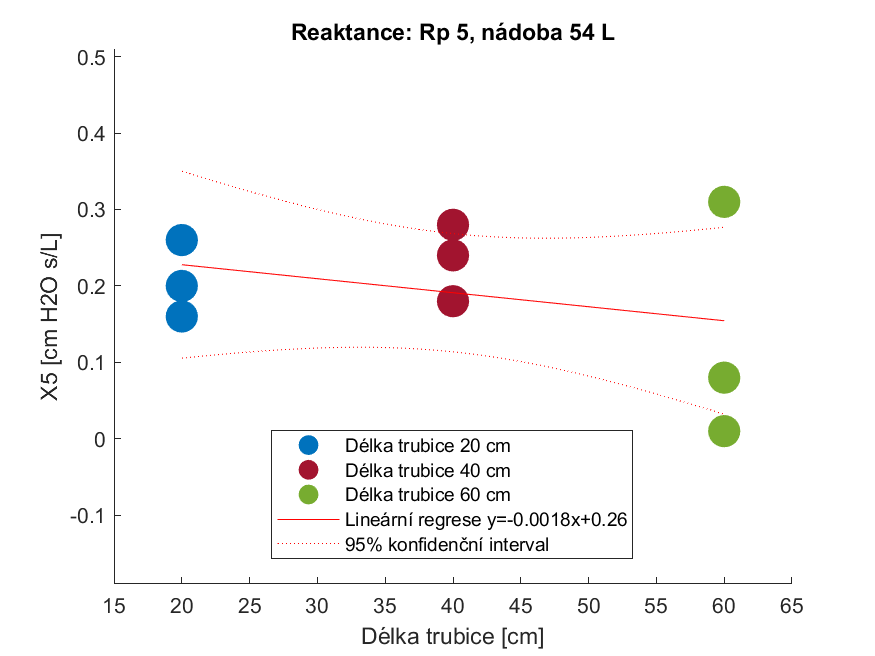
\includegraphics[width=1\linewidth]{reaktance_odpor_5_nadoba_54}
\captionsetup{justification=centering}
   \captionof{figure}{Reaktance: Rp~$\SI{5}{}$,~nádoba~$\SI{54}{L}$}
\end{minipage}
\end{figure}

\begin{figure}
\centering
\begin{minipage}{.5\textwidth}
  \centering
  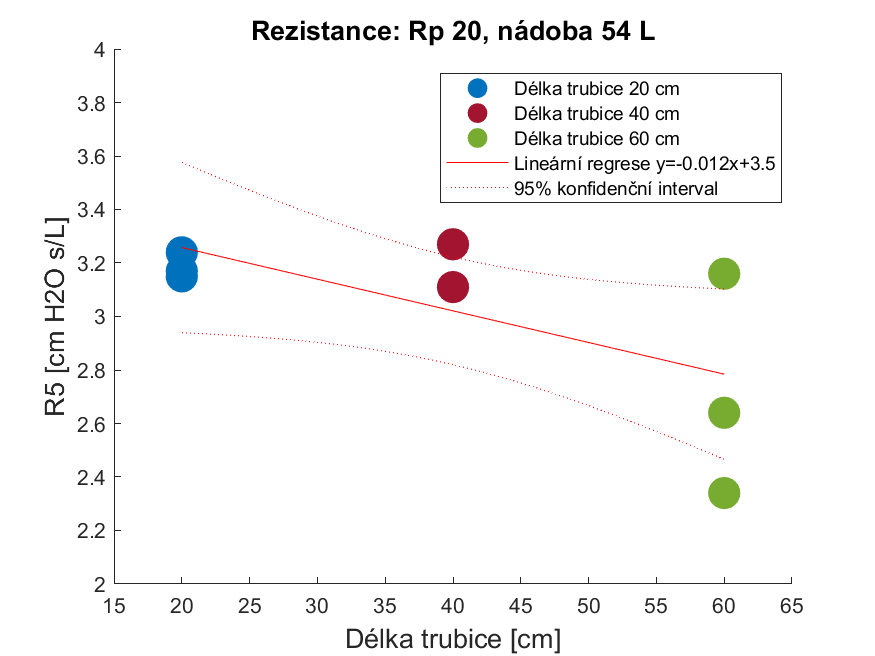
\includegraphics[width=1\linewidth]{rezistance_odpor_20_nadoba_54}
\captionsetup{justification=centering}
  \captionof{figure}{Rezistance: Rp~$\SI{20}{}$,~nádoba~$\SI{54}{L}$}
\end{minipage}%
\begin{minipage}{.5\textwidth}
  \centering
  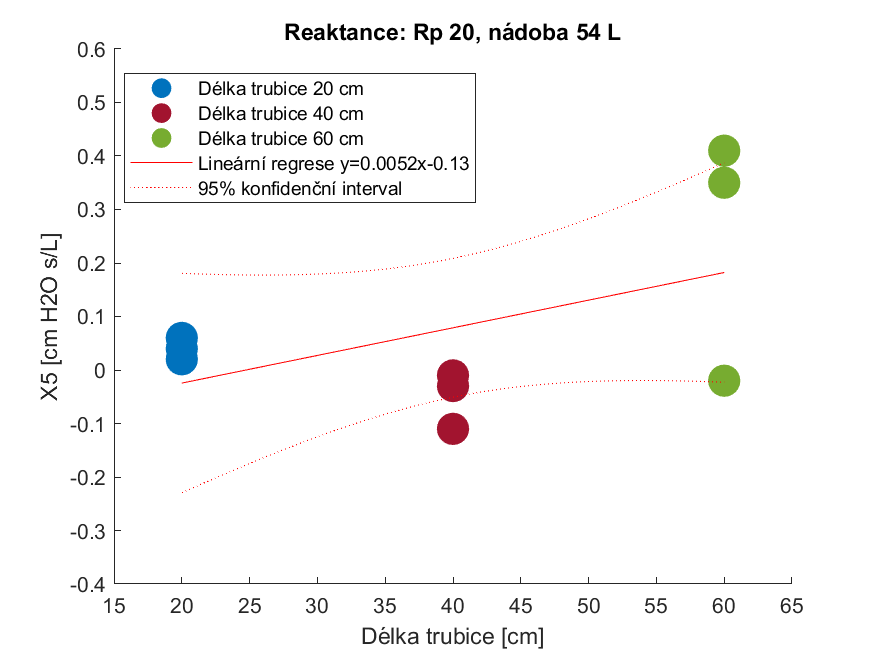
\includegraphics[width=1\linewidth]{reaktance_odpor_20_nadoba_54}
\captionsetup{justification=centering}
   \captionof{figure}{Reaktance: Rp~$\SI{20}{}$,~nádoba~$\SI{54}{L}$}
\end{minipage}
\end{figure}

\begin{figure}
\centering
\begin{minipage}{.5\textwidth}
  \centering
  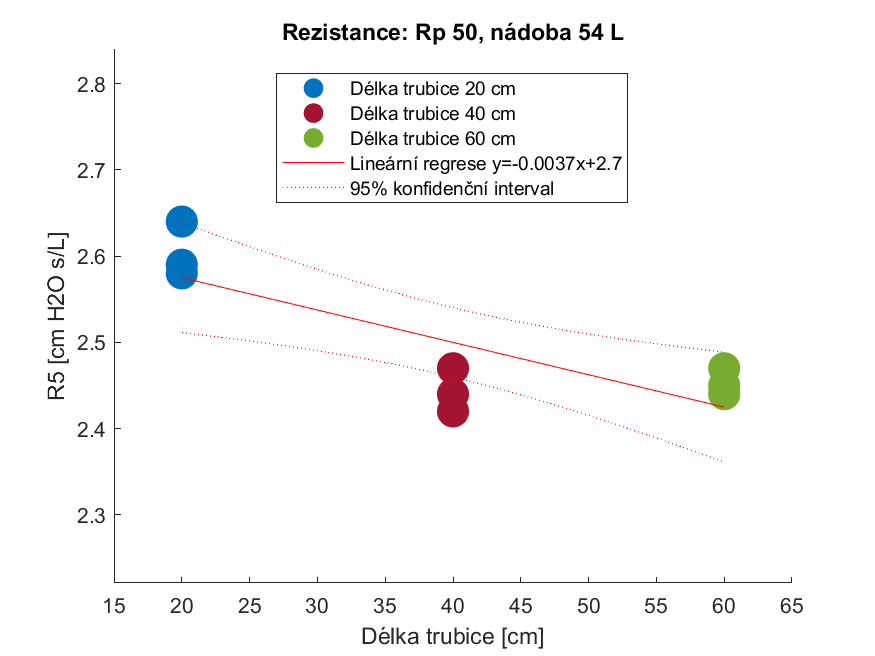
\includegraphics[width=1\linewidth]{rezistance_odpor_50_nadoba_54}
\captionsetup{justification=centering}
  \captionof{figure}{Rezistance: Rp~$\SI{50}{}$,~nádoba~$\SI{54}{L}$}
\end{minipage}%
\begin{minipage}{.5\textwidth}
  \centering
  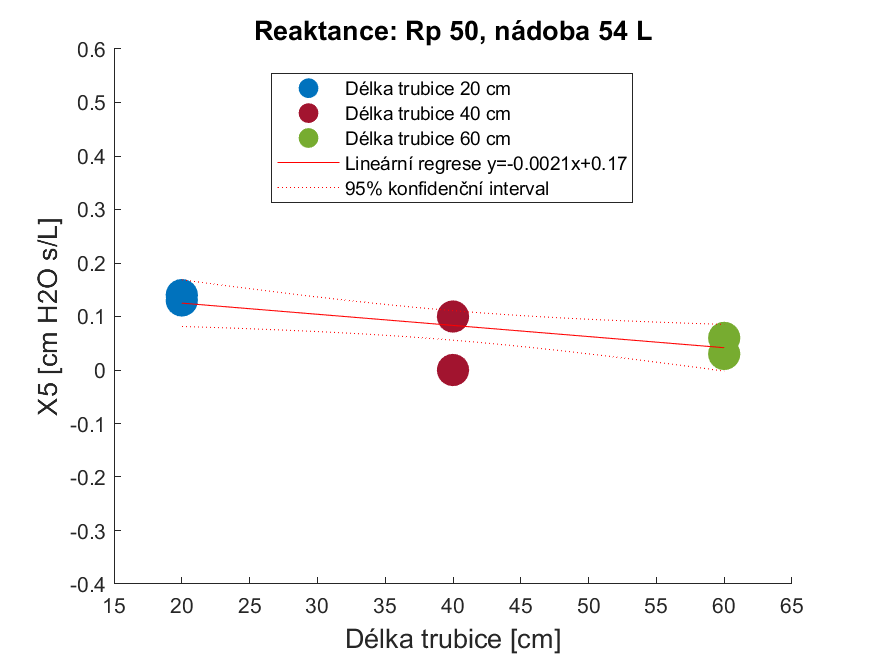
\includegraphics[width=1\linewidth]{reaktance_odpor_50_nadoba_54}
\captionsetup{justification=centering}
   \captionof{figure}{Reaktance: Rp~$\SI{50}{}$,~nádoba~$\SI{54}{L}$}
\end{minipage}
\end{figure}


\begin{figure}
\centering
\begin{minipage}{.5\textwidth}
  \centering
  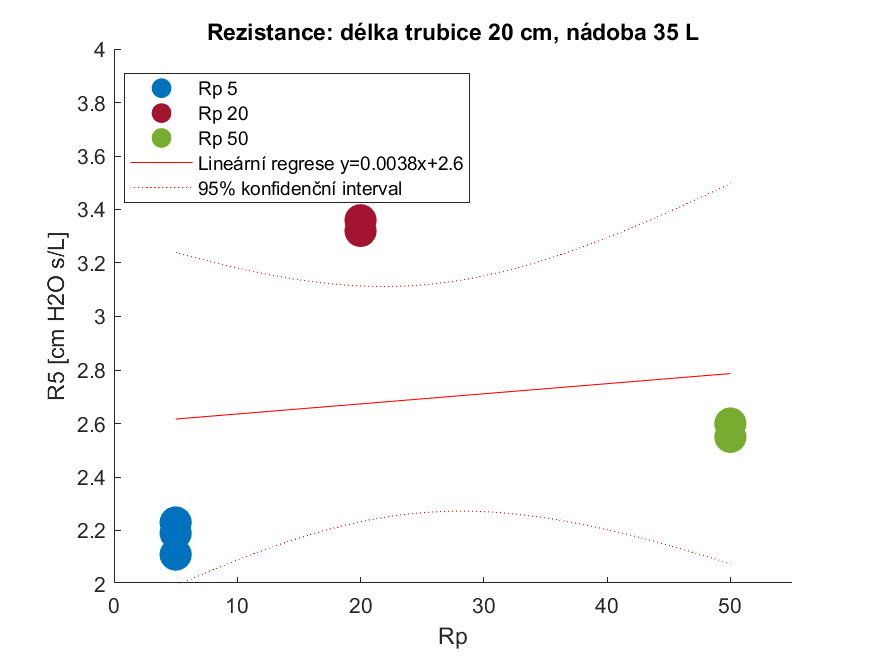
\includegraphics[width=1\linewidth]{rezistance_dily_20_nadoba_35}
\captionsetup{justification=centering}
  \captionof{figure}{Rezistance: délka~trubice~$\SI{20}{cm}$,~nádoba~$\SI{35}{L}$}
\end{minipage}%
\begin{minipage}{.5\textwidth}
  \centering
  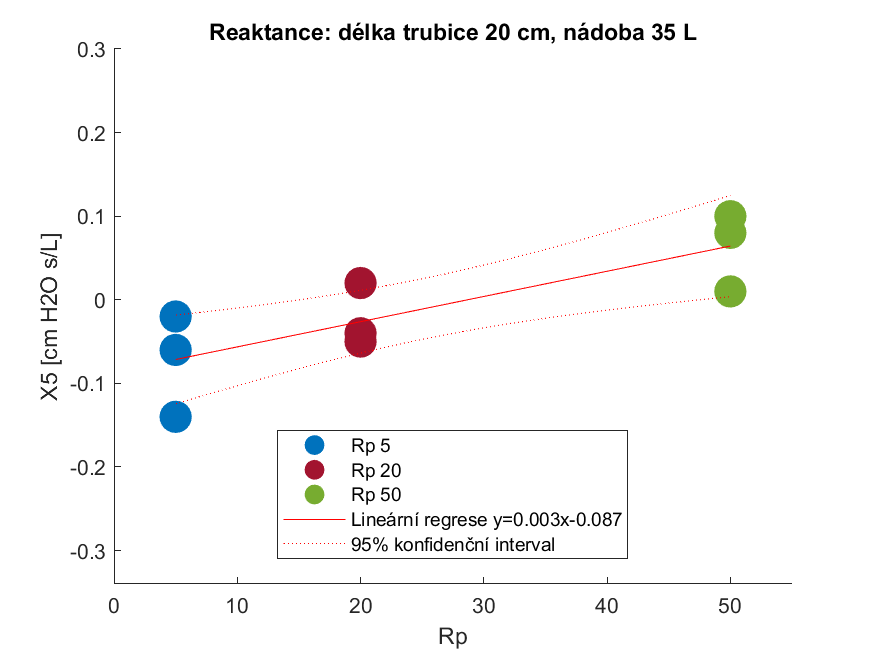
\includegraphics[width=1\linewidth]{reaktance_dily_20_nadoba_35}
\captionsetup{justification=centering}
   \captionof{figure}{Reaktance: délka~trubice~$\SI{20}{cm}$,~nádoba~$\SI{35}{L}$}
\end{minipage}
\end{figure}

\begin{figure}
\centering
\begin{minipage}{.5\textwidth}
  \centering
  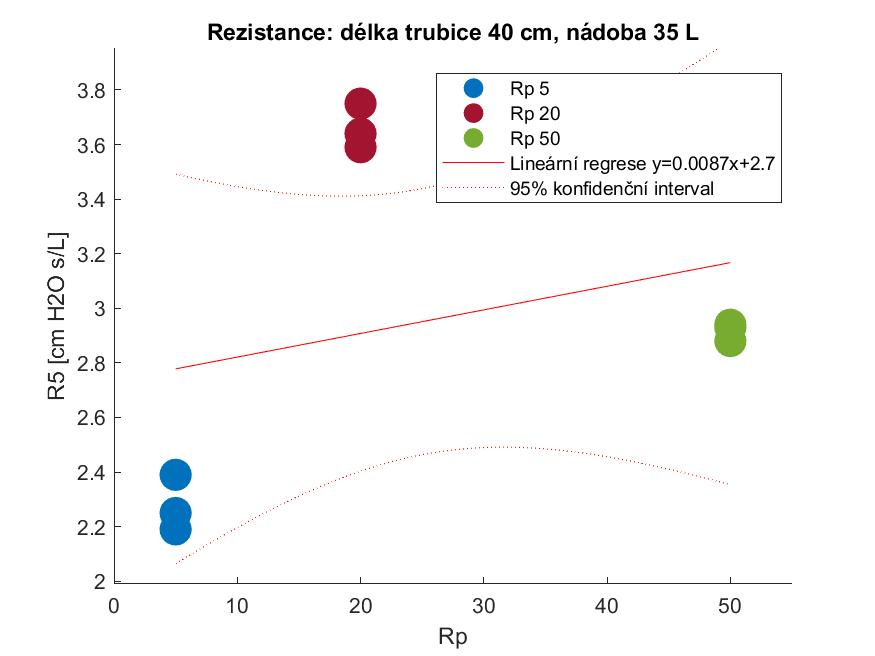
\includegraphics[width=1\linewidth]{rezistance_dily_40_nadoba_35}
\captionsetup{justification=centering}
  \captionof{figure}{Rezistance: délka~trubice~$\SI{40}{cm}$,~nádoba~$\SI{35}{L}$}
\end{minipage}%
\begin{minipage}{.5\textwidth}
  \centering
  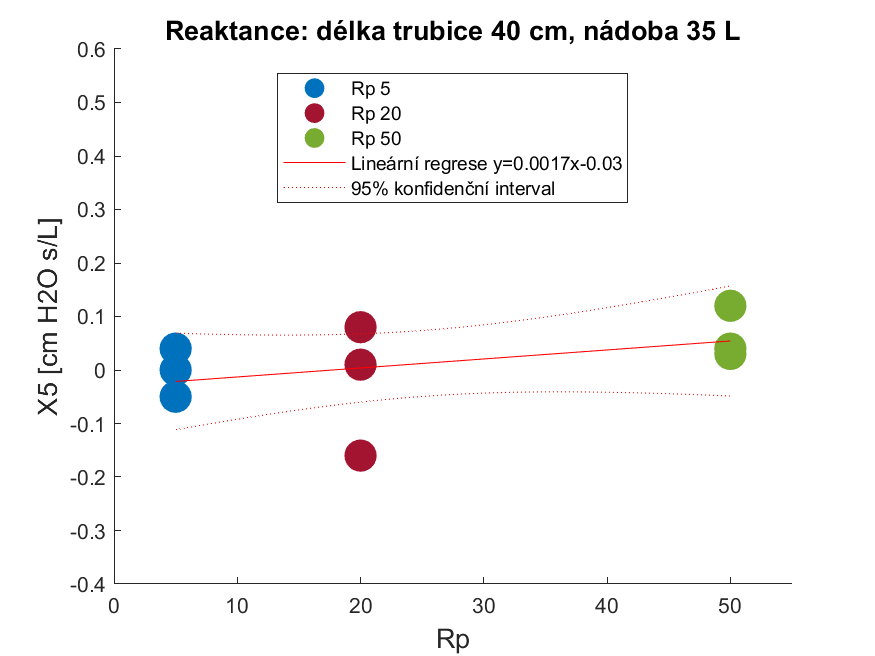
\includegraphics[width=1\linewidth]{reaktance_dily_40_nadoba_35}
\captionsetup{justification=centering}
   \captionof{figure}{Reaktance: délka~trubice~$\SI{40}{cm}$,~nádoba~$\SI{35}{L}$}
\end{minipage}
\end{figure}

\begin{figure}
\centering
\begin{minipage}{.5\textwidth}
  \centering
  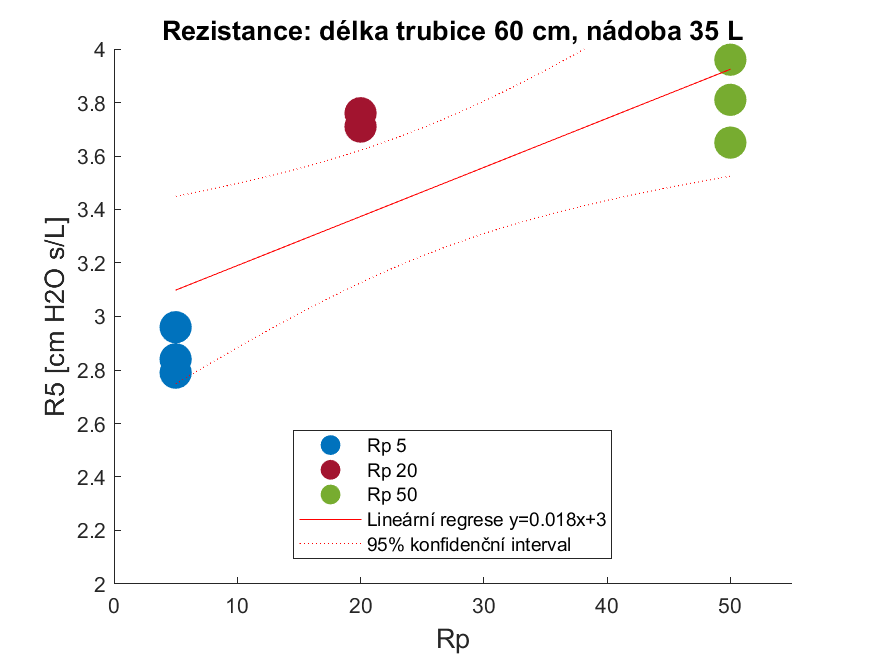
\includegraphics[width=1\linewidth]{rezistance_dily_60_nadoba_35}
\captionsetup{justification=centering}
  \captionof{figure}{Rezistance: délka~trubice~$\SI{60}{cm}$,~nádoba~$\SI{35}{L}$}
\end{minipage}%
\begin{minipage}{.5\textwidth}
  \centering
  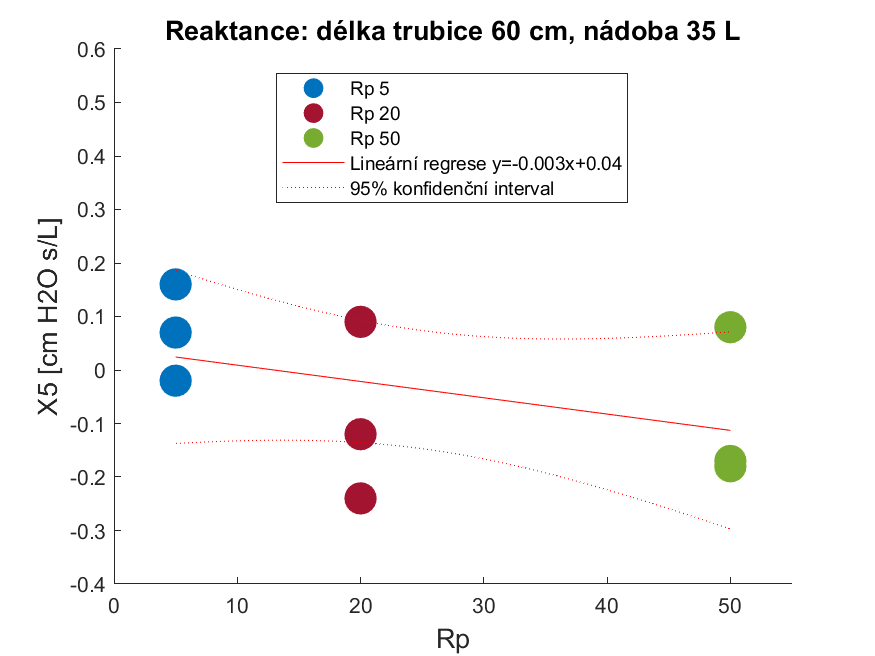
\includegraphics[width=1\linewidth]{reaktance_dily_60_nadoba_35}
\captionsetup{justification=centering}
   \captionof{figure}{Reaktance: délka~trubice~$\SI{60}{cm}$,~nádoba~$\SI{35}{L}$}
\end{minipage}
\end{figure}



\begin{figure}
\centering
\begin{minipage}{.5\textwidth}
  \centering
  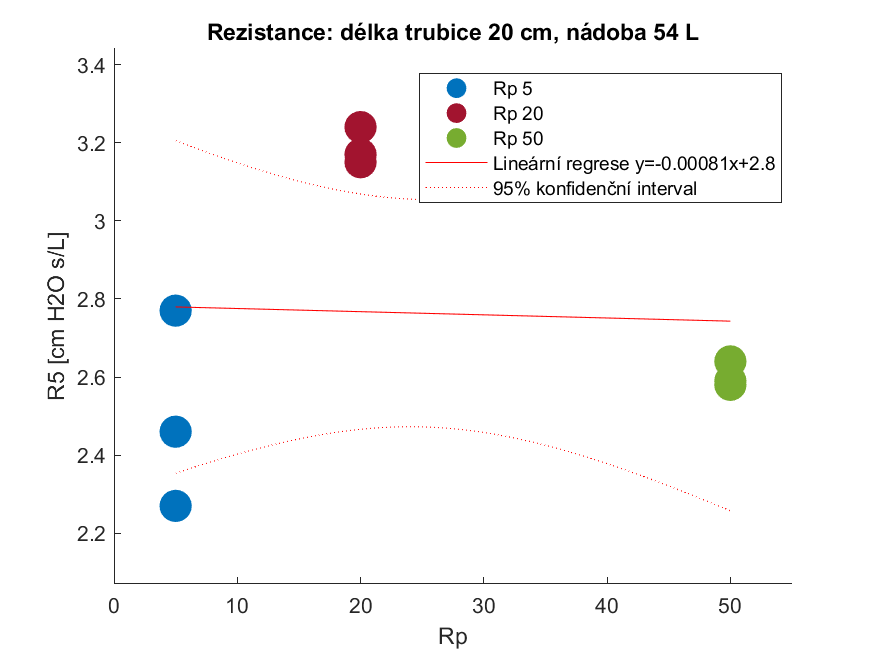
\includegraphics[width=1\linewidth]{rezistance_dily_20_nadoba_54}
\captionsetup{justification=centering}
  \captionof{figure}{Rezistance: délka~trubice~$\SI{20}{cm}$,~nádoba~$\SI{54}{L}$}
\end{minipage}%
\begin{minipage}{.5\textwidth}
  \centering
  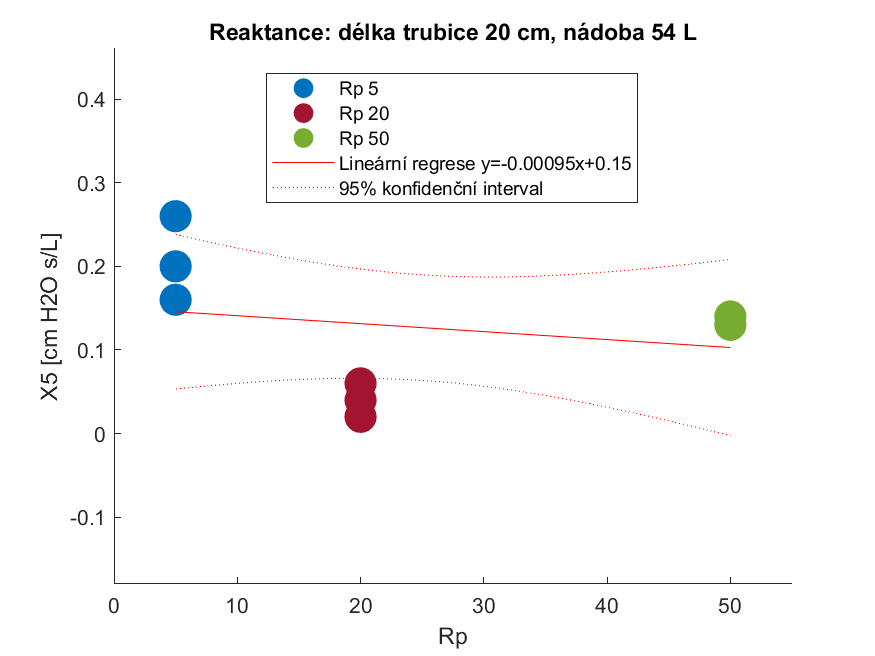
\includegraphics[width=1\linewidth]{reaktance_dily_20_nadoba_54}
\captionsetup{justification=centering}
   \captionof{figure}{Reaktance: délka~trubice~$\SI{20}{cm}$,~nádoba~$\SI{54}{L}$}
\end{minipage}
\end{figure}

\begin{figure}
\centering
\begin{minipage}{.5\textwidth}
  \centering
  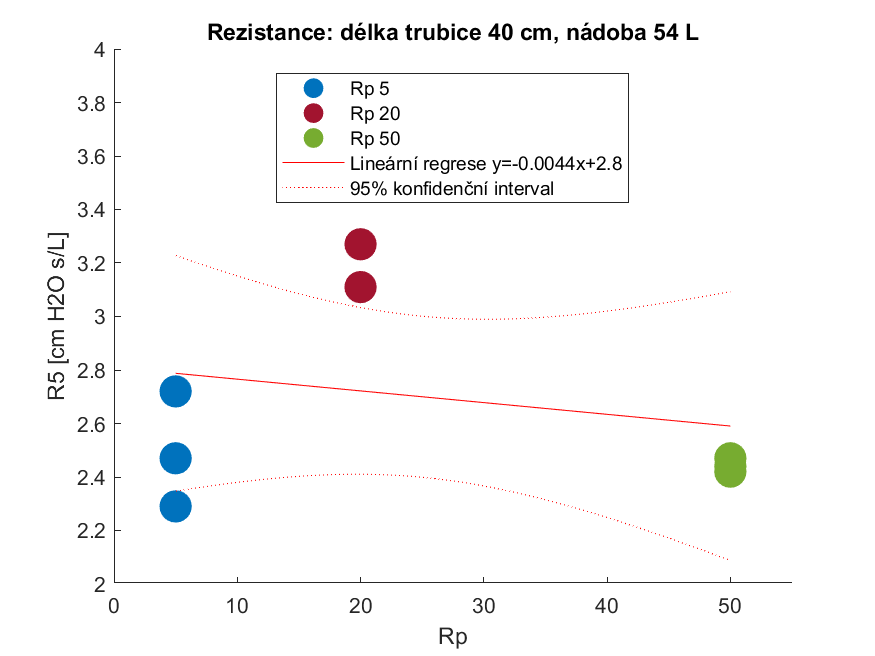
\includegraphics[width=1\linewidth]{rezistance_dily_40_nadoba_54}
\captionsetup{justification=centering}
  \captionof{figure}{Rezistance: délka~trubice~$\SI{40}{cm}$,~nádoba~$\SI{54}{L}$}
\end{minipage}%
\begin{minipage}{.5\textwidth}
  \centering
  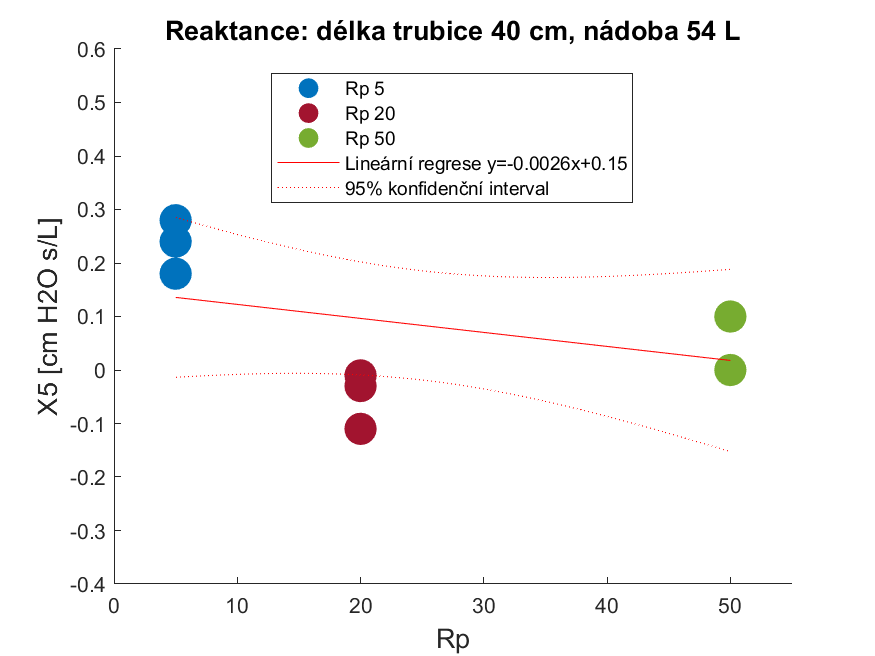
\includegraphics[width=1\linewidth]{reaktance_dily_40_nadoba_54}
\captionsetup{justification=centering}
   \captionof{figure}{Reaktance: délka~trubice~$\SI{40}{cm}$,~nádoba~$\SI{54}{L}$}
\end{minipage}
\end{figure}

\begin{figure}
\centering
\begin{minipage}{.5\textwidth}
  \centering
  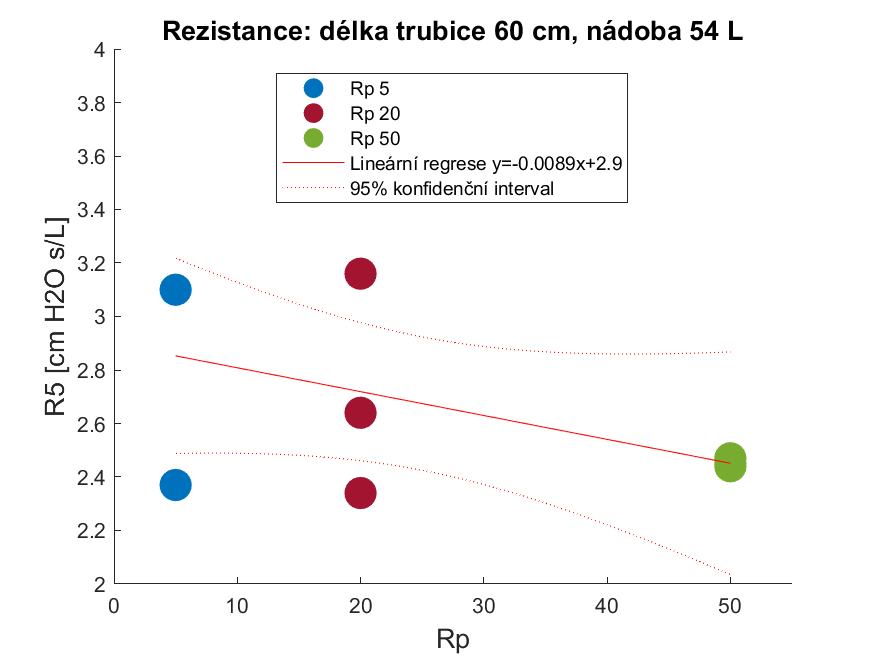
\includegraphics[width=1\linewidth]{rezistance_dily_60_nadoba_54}
\captionsetup{justification=centering}
  \captionof{figure}{Rezistance: délka~trubice~$\SI{60}{cm}$,~nádoba~$\SI{54}{L}$}
\end{minipage}%
\begin{minipage}{.5\textwidth}
  \centering
  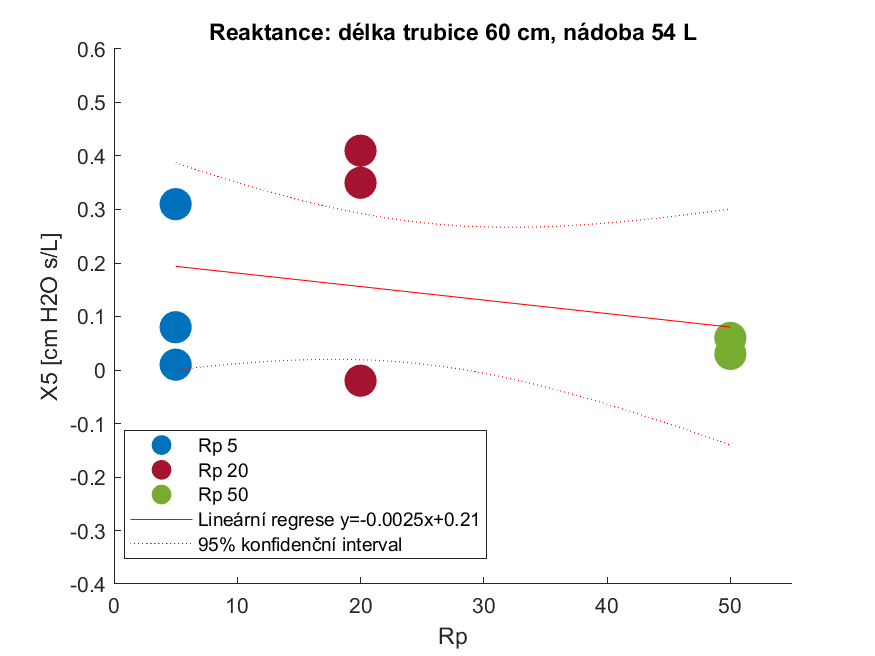
\includegraphics[width=1\linewidth]{reaktance_dily_60_nadoba_54}
\captionsetup{justification=centering}
   \captionof{figure}{Reaktance: délka~trubice~$\SI{60}{cm}$,~nádoba~$\SI{54}{L}$}
\end{minipage}
\end{figure}

	\clearpage
	
	\section{Diskuse}
	
Hlavním cílem práce bylo zjistit závislost zvolených komponent v~modelu respiračního systému na~výsledných naměřených parametrech.  Celkem bylo provedeno 20~různých kombinací 3~velikostí parabolických rezistorů, 3~délek plastových trubic a 2~velikosti skleněných nádob. Měření jsem realizovala pomocí přístroje tremoflo C-100 (Thorasys Thoracic Medical Systems Inc., Kanada) v laboratoři FBMI ČVUT v Praze. 


Do~systému byl v~pravidelných intervalech odpovídajících lidskému dechu vháněn \SI{1}{L} vzduchu, avšak čím byl v~modelu větší rezistor,  tím menší objem byl změřen. U Rp~5 se hodnota objemu pohybovala okolo  \SI{700}{ml}, u Rp~20 kolem  \SI{500}{ml} a u Rp~50 byl změřen objem okolo pouhých \SI{200}{ml}.

Přístroj měří na 8~různých frekvencích, jak bylo již zmíněné v kapitole \ref{kap-metody}. Následně všechny výsledky automaticky uloží do~tabulky. 
Bohužel celá tabulka všech frekvencí nešla vyexportovat, tudíž jsem pracovala pouze s výchozí frekvencí  \SI{5}{Hz}. 

Každá kombinace byla změřena 3x, aby se předešlo nežádoucím nepřesnostem měření. Přestože měření bylo prováděno vícekrát, tak hodnoty pokaždé vycházely s poměrně velkou odchylkou. Největší odchylka vznikala u~měření objemu. 
V~grafech v kapitole~\ref{kap-vysledky} jsem záměrně zvolila stejnou osy y pro rezistenci, resp. reaktanci. To umožnilo vizuálně srovnat opakovatelnost měření -  v ideálním případě by v každém grafu měly být hodnoty odpovídající stejné hodnotě nezávislé veličiny na ose x stejné, protože se jednalo o identická měření. Mnohde je tento předpoklad splněný, například graf \ref{rezistance-dily-20-odpor-20}, jinde jsou nekonzistence měření daleko větší, viz například \ref{rezistance_odpor_5_nadoba_54}.
U rezistence je největší rozptyl kolem $\SI{1}{ cm\cdot H_{2}O}$ a u reaktace kolem $\SI{0,6}{ cm\cdot H_{2}O}$. 


Ještě méně uspokojivý je ale pozorovaný trend, očekávala jsem, že když například zafixuji velikost nádoby a nakreslím 3 grafy pro různé $R_p$, tak pozorovaný trend, v tomhle případě závislost rezistance na délce trubice bude monotónní, tj vždy buď neklesající nebo nestoupající. To obvykle platí, ale některé série měření tohle nesplňují - viz třeba série měření
\ref{rezistance_dily_40_odpor_5}, \ref{rezistance_dily_40_odpor_20} a \ref{rezistance_dily_40_odpor_50} a to i když měření bylo relativně konzistentní.



	\clearpage
	
	\section{Závěr}
	Semestrální projekt zkoumá vztah mezi jednotlivými kombinacemi modelu a naměřených parametrů rezistance a reaktance.
	\clearpage

%-------------Literatura-------------------
    \clearpage	
    \renewcommand{\refname}{Seznam použité literatury} 	% Přejmenování Reference
    \addcontentsline{toc}{section}{Seznam použité literatury}     % Přidání této kapitoly do obsahu
    \printbibliography
    \clearpage

%-------------Přílohy----------------------
    \begin{appendices}
\section{Výsledky měření}
\midinsert \clabel[tvar1]{Tabulka varianta 1}
\ctable{c|r|r|r|r|r|r}
{
 \hfil         &	$R_{5}$    &	$X_{5}$  & $F_{res}$ &	Reference &	$V_{T}$ & $COH_{5}$ \cr
 \hfil  $Měření$ & $[cm \cdot H_{2}O \cdot s / L]$     &	  $[cm \cdot H_{2}O \cdot s / L]$  &	$[Hz]$  & 	 & [L] 	 &        \crl \tskip4pt
1 &	3,16 &	-0,02 &	5,43 &	18,69 &	0,58 &	0,98 \cr
2 &	2,64 &	0,41 &	n/a &	18,69 &	0,73 &	0,97 \cr
3 &	2,34 &	0,35 &	n/a &	18,69 &	0,73 &	0,98 \cr
}
\caption/t Díly: 3, odpor: 20, nádoba: 54	
\endinsert


\midinsert \clabel[tvar2]{Tabulka varianta 2}
\ctable{c|r|r|r|r|r|r}
{
 \hfil         &	$R_{5}$    &	$X_{5}$  & $F_{res}$ &	Reference &	$V_{T}$ & $COH_{5}$ \cr
 \hfil  $Měření$ & $[cm \cdot H_{2}O \cdot s / L]$     &	  $[cm \cdot H_{2}O \cdot s / L]$  &	$[Hz]$  & 	 & [L] 	 &        \crl \tskip4pt
1 &	2,37 &	0,31 &	n/a	 &18,69	 &0,72	 &0,98\cr
2 &	3,1	& 0,01 &	n/a	 &18,69	 &0,51 &	0,99\cr
3 &	3,1	& 0,08 &	n/a &	18,69 &	0,47 &	0,99\cr
}
\caption/t Díly: 3, odpor: 5, nádoba: 54	
\endinsert


\midinsert \clabel[tvar3]{Tabulka varianta 3}
\ctable{c|r|r|r|r|r|r}
{
 \hfil         &	$R_{5}$    &	$X_{5}$  & $F_{res}$ &	Reference &	$V_{T}$ & $COH_{5}$ \cr
 \hfil  $Měření$ & $[cm \cdot H_{2}O \cdot s / L]$     &	  $[cm \cdot H_{2}O \cdot s / L]$  &	$[Hz]$  & 	 & [L] 	 &        \crl \tskip4pt
1&	2,47&	0,06&	n/a	&    18,69&	0,23&	1\cr
2&	2,44&	0,03&	n/a&	18,69&	0,22&	1\cr
3&	2,45&	0,06&	n/a&	18,69&	0,24&	1\cr
}
\caption/t Díly: 3, odpor: 50, nádoba: 54	
\endinsert


\midinsert \clabel[tvar4]{Tabulka varianta 4}
\ctable{c|r|r|r|r|r|r}
{
 \hfil         &	$R_{5}$    &	$X_{5}$  & $F_{res}$ &	Reference &	$V_{T}$ & $COH_{5}$ \cr
 \hfil  $Měření$ & $[cm \cdot H_{2}O \cdot s / L]$     &	  $[cm \cdot H_{2}O \cdot s / L]$  &	$[Hz]$  & 	 & [L] 	 &        \crl \tskip4pt
1&	2,47&	0,1	&n/a&	18,69&	0,27&	1\cr
2&	2,42&	0&	n/a	&18,69&	0,24&	1\cr
3&	2,44&	0,1&	n/a&	18,69&	0,22&	1\cr
}
\caption/t Díly: 2, odpor: 50, nádoba: 54	
\endinsert


\midinsert \clabel[tvar5]{Tabulka varianta 5}
\ctable{c|r|r|r|r|r|r}
{
 \hfil         &	$R_{5}$    &	$X_{5}$  & $F_{res}$ &	Reference &	$V_{T}$ & $COH_{5}$ \cr
 \hfil  $Měření$ & $[cm \cdot H_{2}O \cdot s / L]$     &	  $[cm \cdot H_{2}O \cdot s / L]$  &	$[Hz]$  & 	 & [L] 	 &        \crl \tskip4pt
1&	3,24&	0,04&	n/a	&18,69&	0,53&	0,99\cr
2&	3,15&	0,02&	n/a	&18,69&	0,57&	0,98\cr
3&	3,17&	0,06&	n/a&	18,69&	0,54&	0,99\cr
}
\caption/t Díly: 1, odpor: 20, nádoba: 54	
\endinsert



\end{appendices}



    
\end{document}